\renewcommand{\bf}{\bfseries}

\chapter{Cherenkov Optical Calibration Source for SNO+}
\label{ch:chsrc}

SNO+ has over 9500 Photo-Multiplier Tubes (PMTs), which detect photons produced inside the target (water or liquid scintillator).
Within the SNO+ calibration plan~\cite{gann:2013} it is vital to extract and monitor the overall light collection efficiency of these PMTs, because this determines the energy response of the detector.
The Cherenkov source was designed to produce a well understood optical signal, which can be used to measure these quantities.

The Cherenkov source is able to make the measurements in a way nominally independent of the target as described in \Cref{chap:motivation}. 
The detailed design of the source is discussed in \Cref{chap:design}. 
The construction procedures are briefly covered in \Cref{chap:construction}.
Tests  \Cref{chap:tests}.
Finally \Cref{chap:water_phase} discusses the deployment of this source in SNO+ water phase and an analysis of the data taken during the deployment.

\section{Motivation}
\label{chap:motivation}

For both Chernekov and scintillation light, visible energy is proportional to the total number of generated photons.
In the case of a water target, the production of Cherenkov light is well understood and can be accurately simulated from first principles.
In order to calibrate the energy response of the detector, a radioactive source with a well understood energy spectrum, such as an \N source, can be deployed and used to calibrate a simulation model.
In this case, with Cherenkov production being simulated accurately, only the response of the detector needs to be tuned in simulation to reproduce the data.

When SNO+ switches to liquid scintillator, this situation is more complicated because the scintillation process is not as easy to model.
For instance, the photon yield typically must be measured for any independent batch of scintillating liquid, whereas the production of Cherenkov light is calculable. 
This means that calibrating the energy scale of the detector with something like an \N source would be unable to disentangle changes to scintillation output from changes in detector response.
Disentangling these two effects can be achieved by deploying a source that produces a well understood and easily simulated optical signal. 
The Cherenkov source is designed to produce such a signal through tagged Cherenkov events.


\section{Source Design}
\label{chap:design}

The Cherenkov light produced by this source will come from stopping beta decay electrons from \Li in UV-absorbent (UVA) acrylic, and is based on the SNO \Li source design and experience~\cite{Tagg:2002,Tagg:2001}.
The choice of UVA acrylic was made to block the UV component of Cherenkov light, which would be absorbed and reemitted by the scintillator.
Thus, the remaining light that propagates through the SNO+ detector is quasi-independent of the optical properties of the LAB-PPO scintillator. 
This visible Cherenkov light is easy to model, allowing for a measurement of detector response nominally independent of the target material.

\begin{figure}[]
\center{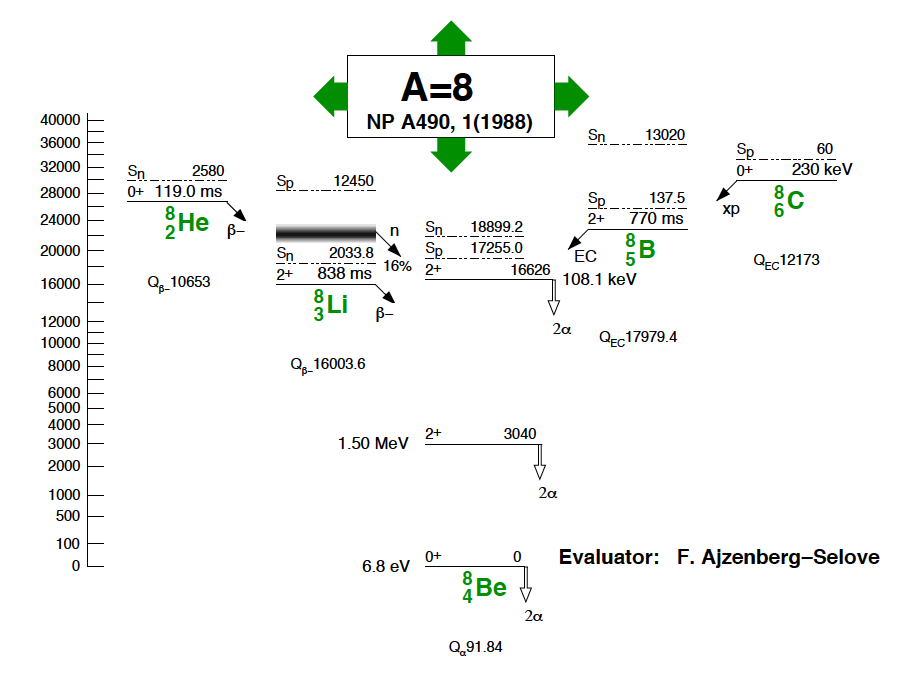
\includegraphics[width=.7\textwidth]{Ais8DecayScheme.png}}
\caption{\label{fig:decayscheme} A=8 decay scheme. Taken from~\cite{Tagg:2001}.}
\end{figure}

The decays following \Li in the decay chain (see \Cref{fig:decayscheme}) results in a very fast alpha decay following the production of the beta.
The chamber in which the decay occurs will be filled with helium gas in which these alphas will produce scintillation light.
This scintillation light is hard UV, around 80-nm, and impossible for traditional PMTs to detect, so the chamber will contain a wavelength shifter,  Tetraphenyl Butadiene (TPB), to convert the UV photons to approximately 420-nm light.
These shifted photons can then be detected by an internal PMT to produce a tag signal for the primary \Li decays.

Because this is a calibrated light source, any other processes that may produce optical photons should be well understood and, where possible, eliminated with design choices.
The alpha scintillation, especially including the wavelength shifted photons, must be contained within the source. 
Additionally, any energetic particles produced in the \Li decay must be taken into account.
The UVA acrylic is designed thick enough to stop all of the \Li betas from exiting, however, these energetic electrons can produce Bremsstrahlung gammas that do escape the source.
When deployed in water phase these gammas will not produce sufficient light to interfere with analysis of the data, however, in scintillator phase these will be a significant background to the measurement, and must be cut in an offline analysis. 

\subsection{Cherenkov Event Generation}

The \Li (t$_{1/2}$=0.838\,s) isotope is created using a deuterium-tritium neutron generator in conjunction with a $^{11}$B target.
Neutron captures on $^{11}$B produce $^{12}$B, which alpha decays to \Li.
The \Li is transported by helium gas to the spherical decay chamber at the center of the source as shown in Figure~\ref{fig:design-1}. 
The energetic beta particles produced by the decay are stopped in the 6\,cm-thick spherical acrylic wall and produce Cherenkov light. 
The alphas from the subsequent $^{8}$Be decay produce scintillation light in the helium, which is then wavelength shifted by TPB present in the lining of the decay chamber.
A small PMT in the neck of the source detects this scintillation light, generating a tagging signal for the event. 

\subsection{Source Geometry}
The Cherenkov source consists of three main parts: the acrylic decay chamber, the PMT assembly inside the neck, and the steel housing inherited from the SNO \Li source. See Figures~\ref{fig:design-1} and~\ref{fig:design-2}.
See~\cite{wallig:2015} for the complete set of technical drawings for the Cherenkov source. 3D-rendered drawings are used in this section to identify the different parts of the source.

\begin{figure}
\center{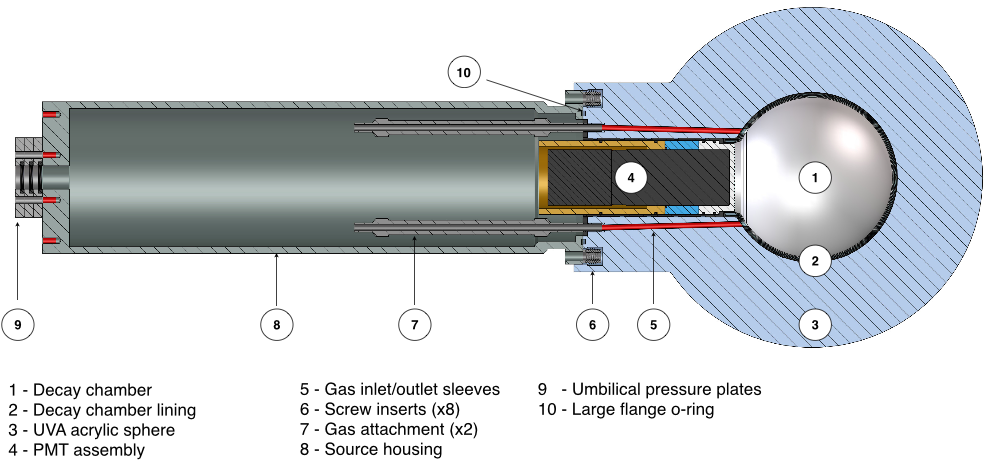
\includegraphics[width=1.0\textwidth]
{Design-1.png}}
\caption{\label{fig:design-1}Schematic of the fully assembled Cherenkov source.}
\end{figure}

\begin{figure}
\center{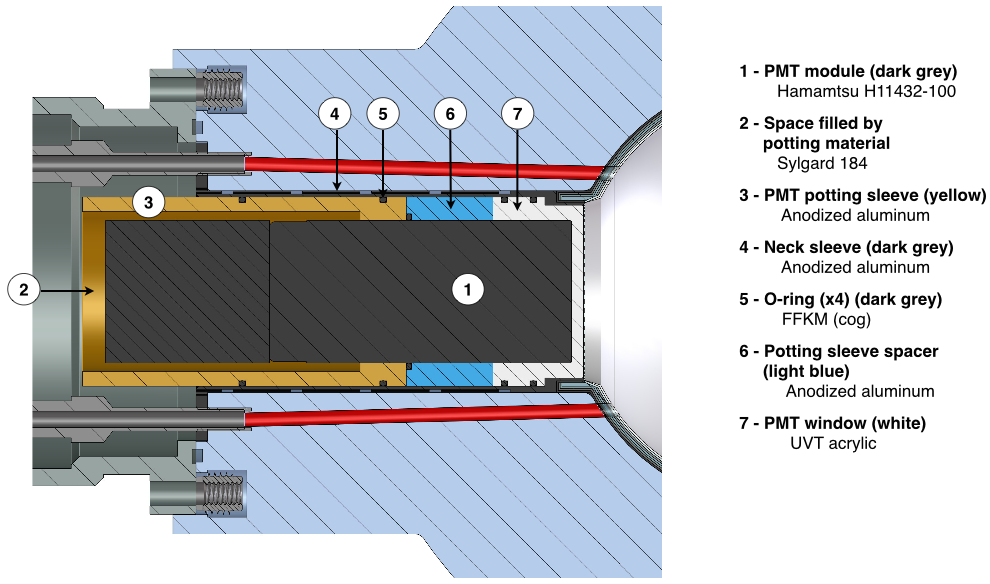
\includegraphics[width=1.0\textwidth]
{Design-2.png}}
\caption{\label{fig:design-2}Detail of the PMT assembly.}
\end{figure}

\subsubsection{Decay chamber}

The decay chamber is roughly a sphere made out of UVA acrylic supplied by RPT (Reynolds Polymer Technology). 
This is machined in two halves, which must be bonded using Weld-on\,\#40. Details on this procedure are found in \Cref{sec:bond}.
The inside of the decay chamber is lined with an opaque, reflective and wavelength-shifting coating, which consists of 4 layers of paint, which are discussed further in \Cref{sec:lining}.
A thin neck-sleeve made from anodized aluminum is potted in place using Sylgard 184 to accept the tag PMT assembly. 
It serves to ensure light-tightness, specifically around the PMT window.
Two thin steel capillaries are potted inside the gas inlet and outlets holes with Sylgard~184. These are needed in order to ensure light-tightness and do not form gas seals. The inlet lines are threaded into the acrylic and the threads are potted in with Sylgard~184. 
The attachement of the decay chamber to the steel housing is done by way of 8 stainless steel screws. 8 screw-inserts are glued in place inside the top of the decay chamber using Weld-on\,\#40.
A single large o-ring is placed in the plane where the steel housing is connected to the decay chamber. 
This seal prevents target material ingress into the source body, while the decay chamber is further isolated by a second set of o-ring seals.

\subsubsection{PMT assembly}

The PMT module fits inside the neck to observe the scintillation light inside the decay chamber. 
The module is a Hamamatsu H11432-100, which has an integrated high voltage supply that requires only low voltage (+5V) to operate. 
This module is potted into an anodized aluminum holder (\cite{wallig:2015}, page 8) using a silicone encapsulate Sylgard~184. 
On the front of this PMT module is a UVT acrylic window that faces into the decay chamber. This is intended to contain the helium gas while allowing the wavelength shifted tag signal photons to reach the tag PMT.
There are 4 small o-rings between the PMT assembly and the neck-sleeve, they are made from FFKM material.

\subsubsection{Steel housing}
The housing (\cite{wallig:2015}, page 12) and the gas connections (\cite{wallig:2015}, page 13) are inherited from the SNO \Li source. 
The housing is made of stainless steel and can be shortened if needed. 
To handle the different types of connections used in different phases of SNO+, a flange was added to the original steel housing, as shown in Figure~\ref{fig:flange}. 
The gas connections can also be changed if needed by modifying the gas lines threaded into the decay chamber.
The steel housing is electropolished and cleaned to remove any surface contaminates before the final assembly and deployment of the source.

\begin{figure}
\center{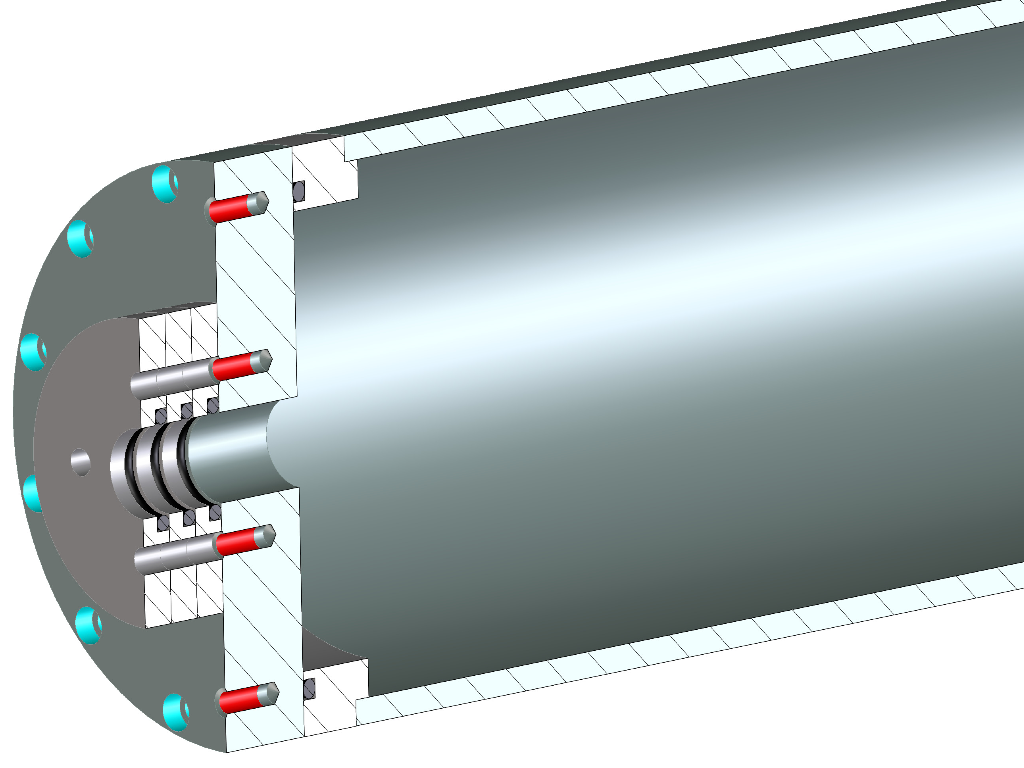
\includegraphics[width=.5\textwidth]
{flange.png}}
\caption{\label{fig:flange} Schematic of a suggested flange to be welded at the top of the source housing. }
\end{figure}

\subsection{Deployment hardware}

For deployment during the SNO+ water-phase, the SNO \Li umbilical to transport \Li into the source was re-used.
Figure~\ref{fig:sno_umbilical} shows the cross-section of this umbilical. It contains the required gas-transport lines in addition to the electrical wires; one for the PMT signal and three for the low-voltage for the PMT (ground, power, control voltage). 
The umbilical currently has no connector. 
Just as was done for SNO, the plan is to connect the gas hoses and wiring for the PMT by hand while the top of the source (steel housing) is exposed. 
Then the sealing pressure plates (Figure~\ref{fig:pressureplates}) are slid down and bolted together. 
The so-called 'lighthouse' attachment, see Figure~\ref{fig:connection}, sits on the endcap and is used to attach the source to SNO+'s source deployment hardware.

\begin{figure}
\begin{subfigure}{.57\textwidth}
\center{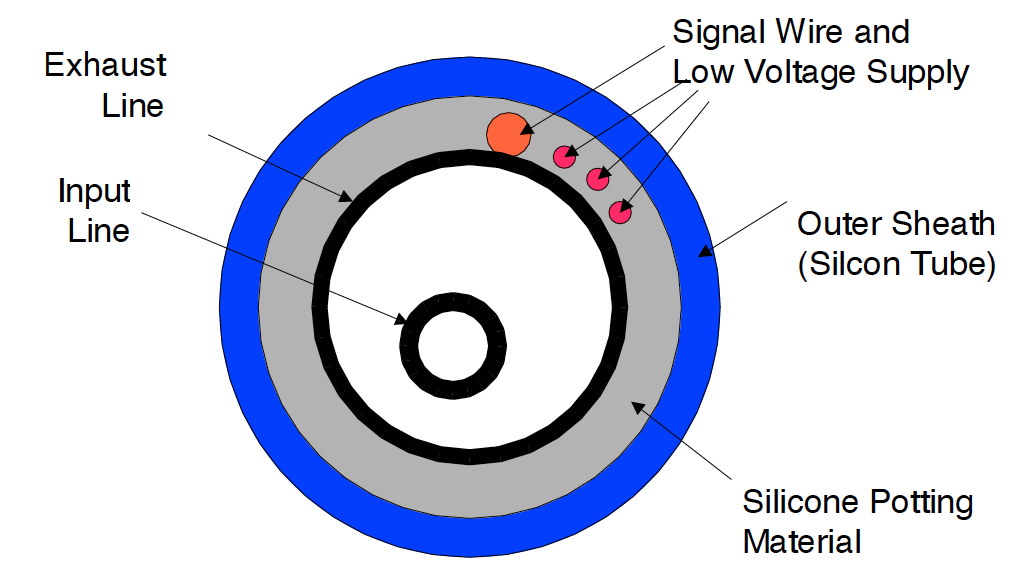
\includegraphics[width=1.0\textwidth]
{8Li-Umbilical.png}}
\caption{\label{fig:sno_umbilical} The SNO \Li umbilical cross-section. Taken from~\cite{Tagg:2001}.}
\end{subfigure}
\hspace{0.5cm}
\begin{subfigure}{.35\textwidth}
  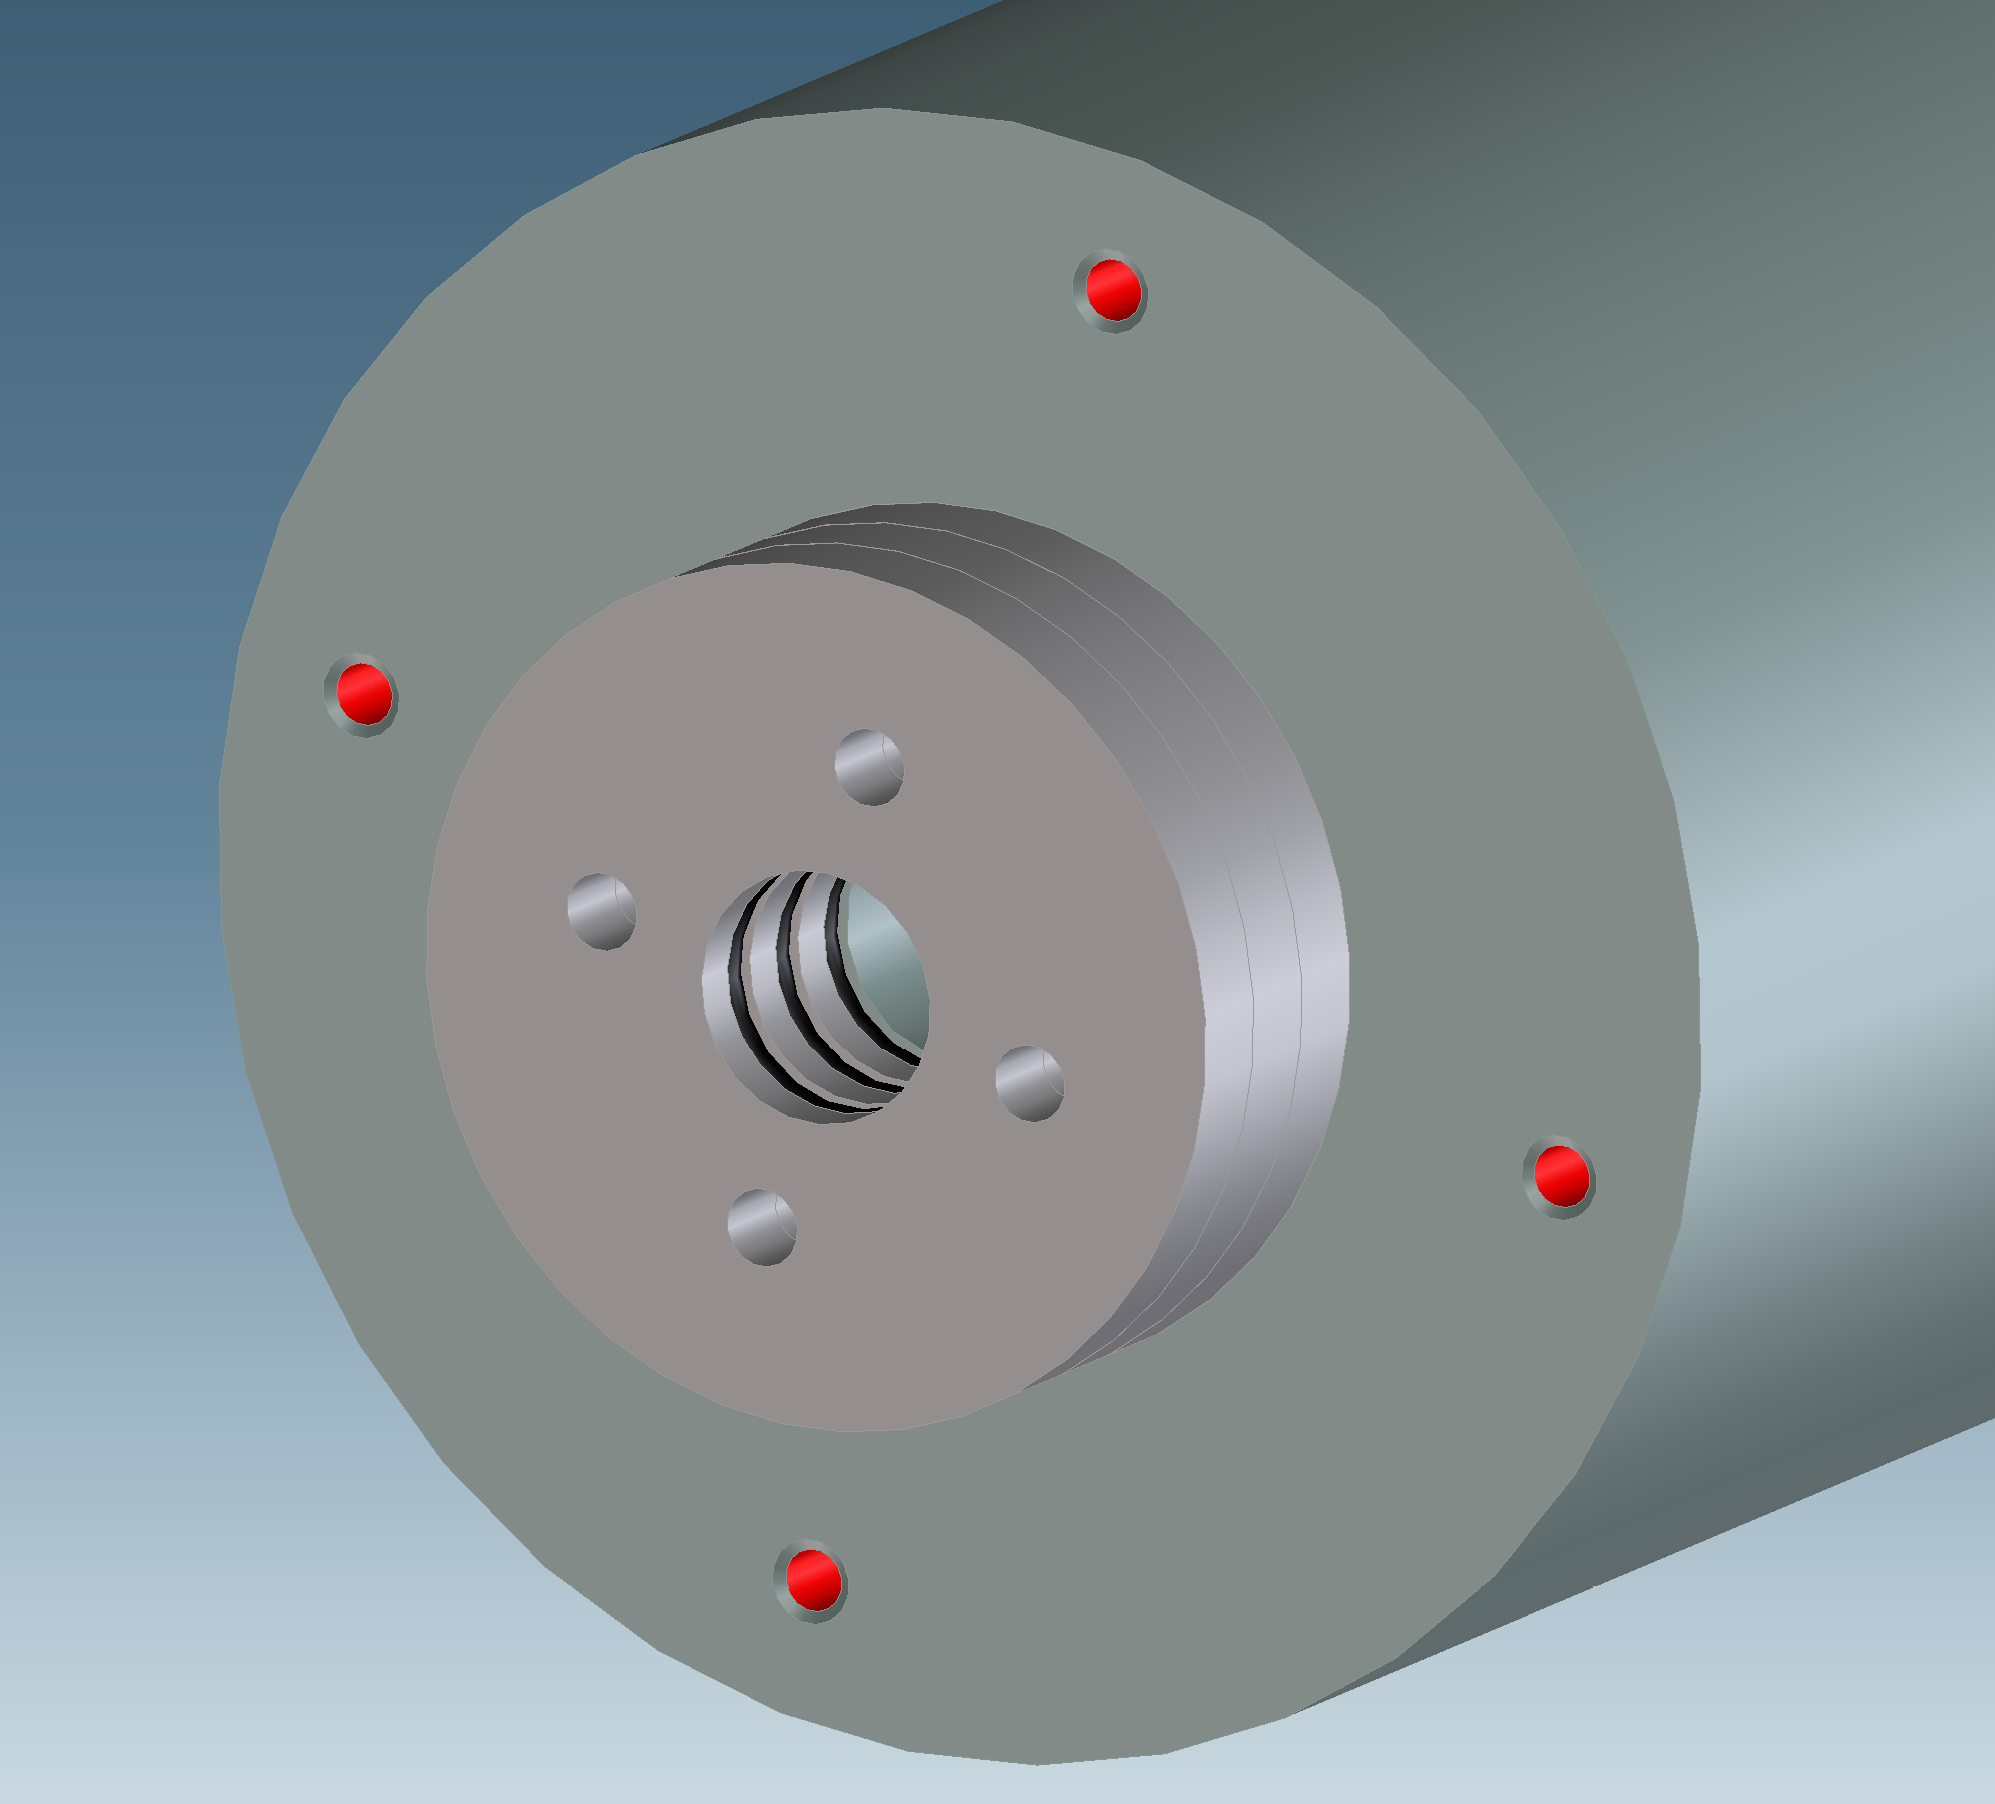
\includegraphics[width=\textwidth]{HousingTop.png}
  \caption{\label{fig:pressureplates} The sealing pressure plates.}
\end{subfigure}
\caption{Details of the umbilical and the water-phase umbilical connection to the source housing.}
\end{figure}

\begin{figure}
\center{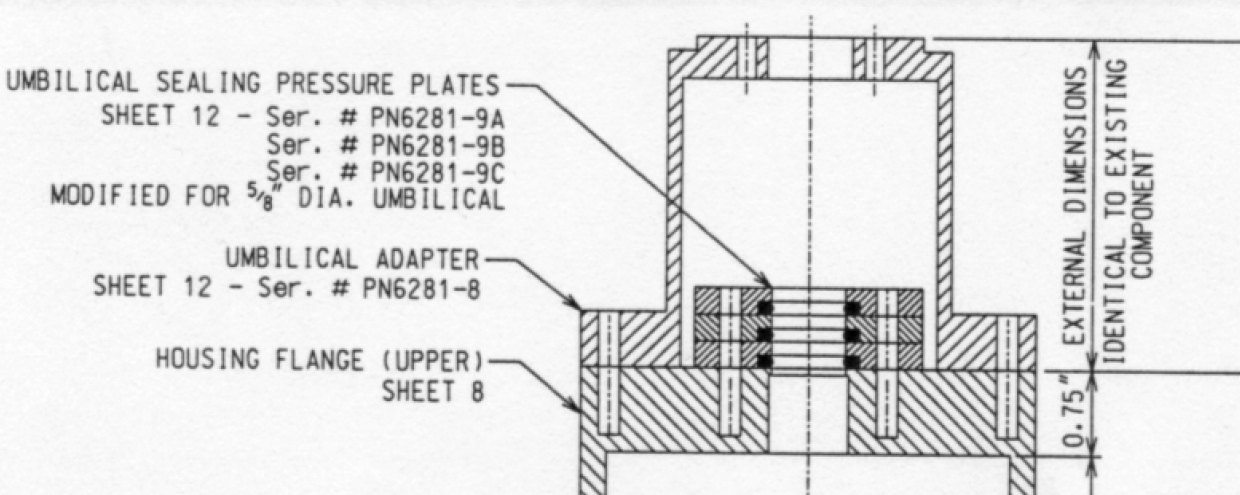
\includegraphics[width=.8\textwidth]
{UmbilicalConnection.png}}
\caption{\label{fig:connection}Detail of the SNO \Li technical drawing, showing the top assembly with the pressure plates and the 'lighthouse'. Taken from~\cite{Tagg:2001}.}
\end{figure}

The umbilical that will be used for deployment in the liquid scintillator still needs to be produced. 
It is expected to be of a similar design as the SNO \Li umbilical with the difference that there will be a source connector permanently attached to the umbilical. 
An adapter then needs to be designed to connect to the Cherenkov source. 

\section{Decay Chamber Construction}
\label{chap:construction}

The Cherenkov source decay chamber is a hollow acrylic sphere.
It is formed out of two acrylic slabs that are bonded together.
The annealing, bonding, decay chamber lining and PMT potting are described in the next sections.
The bonding, painting and storage of the decay chamber was done inside a class-1000 clean room at LBNL.
The construction of the Cherenkov source decay chamber has roughly the following steps:

\begin{enumerate}
    \item Pre-anneal: the acrylic is pre-annealed at the production site (RPT).
    \item Machine cycle 1 (see~\cite{wallig:2015}, page 2): hollow out the decay chamber and neck from the two slabs. Machine holes for alignment pins. 
    \item Polish: the inside of the decay chamber is polished using NOVUS heavy and fine scratch remover (Diatomaceous earth/Silica)~\cite{polish}. 
    \item Sand: the bond-plane is sanded to prepare for the bond using NORTON Blue-Bak waterproof paper (Silicon carbide) grit, 220, 320, 400, 600~\cite{sand}.
    \item Ultra high vacuum cleaning.
    \item Anneal: the two machined slabs are annealed.
    \item Ultra high vacuum cleaning.
    \item Mask: masking paint (Micro Mask MI-7~\cite{masking}) is used to protect the inside of the decay chamber from the cement. This product is easily removed with water.
    \item Bonding: bond the two halves together using Weld-on \#40, an acrylic cement. 
    \item Remove masking: once the cement has set, remove the masking from the inside of the decay chamber.
    \item Machine cycle 2 (see~\cite{wallig:2015}, pages 5 and 6): remove excess acrylic to form sphere, drill the gas inlet/outlet holes, machine o-ring groove.
    \item Ultra high vacuum cleaning.
    \item Decay chamber lining: use paints and TPB to line the inside of the decay chamber. This also requires potting of the neck sleeve and gas inlet and outlet sleeves.
    \item PMT potting: pot the tag PMT inside the PMT sleeve.
    \item Assembly and testing.
\end{enumerate}

\subsection{Acrylic Annealing}

Before bonding, the acrylic blocks must be annealed to remove any residual stresses. The annealing process raises the temperature of the acrylic in a controlled way so that stress frozen into the cold solid acrylic can relax away, and then lowers the temperature in a controlled way so that new stress is not developed. This is necessary to ensure that there are no residual stresses that will cause reduced optical clarity (crazing) or mechanical failure (poor bond). The blocks were placed in an annealing oven shown in Figure~\ref{fig:oven} that was programmed to follow an annealing curve containing an initial ramp, a soak phase, and a cool-down ramp. Most information for acrylic annealing was obtained from an Air Force / Navy acrylic fabrication specification MIL-P-6997B(ASG) and the Handbook of Acrylics. The thickness of the acrylic during annealing is 152~mm, which is used for calculating the lengths of the annealing stages, and a soak temperature of 80\degree C was chosen to ensure the acrylic can relax without risking deformation of the machined surfaces. The final annealing curve is shown in Figure~\ref{fig:annealing}.

\begin{figure}
\begin{subfigure}{.54\textwidth}
  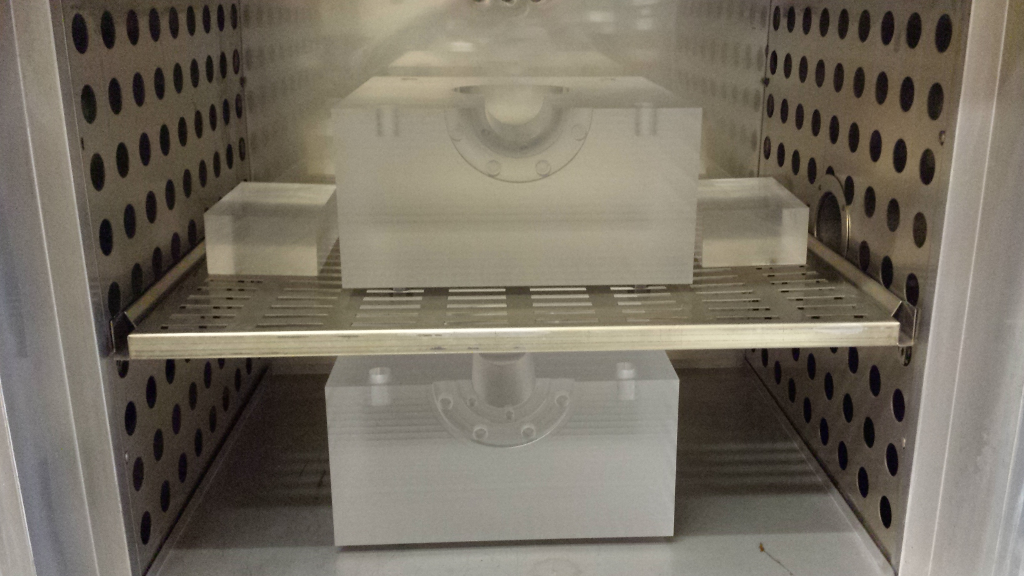
\includegraphics[width=\textwidth]{annealing_oven.png}
  \caption{Source and reference-block acrylic in oven.}
  \label{fig:oven}
\end{subfigure}
\begin{subfigure}{.47\textwidth}
  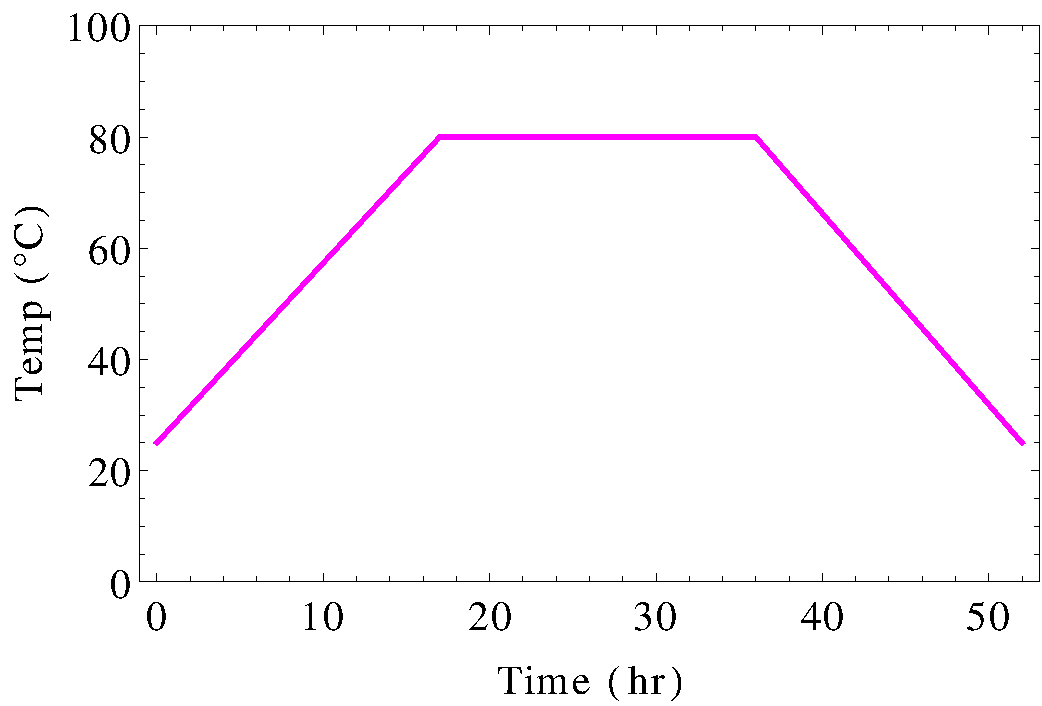
\includegraphics[width=\textwidth]{annealing_curve}
  \caption{51 hour annealing cycle.}
  \label{fig:annealing}
\end{subfigure}
\caption{Acrylic must be annealed to allow any residual stresses that may result in optical flaws post-bonding to relax away.}
\label{fig:annealfig}
\end{figure}

\subsection{Bonding of the Decay Chamber}
\label{sec:bond}

The bond of the two acrylic slabs is required to be optically flawless, strong and leak-proof. 
After studies of various types of acrylic bonding agents~\cite{tanner:2014}, Weld-On\,\#40 was chosen as the bonding because of the clear advantages over methylene chloride in bond quality and ease of use.
Weld-On\,\#40 has shown to be leak resistant, durable, and slow to cure, which allowed sufficient time to ensure accurate placement of the acrylic blocks. 
Additionally, a Weld-On\,\#40 bond maintains good optical properties, is very strong at room temperature and the slow cure is expected to produce less stress in the acrylic after the bond.

The bonding of the two acrylic blocks that make up the Cherenkov source decay chamber is a critical step in the Cherenkov source construction. 
The procedure for this bonding was developed after many tests and mock-bonding walk-throughs. 
The bonding procedure describes how to safely and cleanly prepare and apply the bonding agent, how to align and clamp the two acrylic pieces together, and how to deal with the excess cement that will leak inside the decay chamber.
It can be found in full in \Cref{chap:bondproc}.
After this step, the source can proceed to the final machining cycle to form the outer spherical surface, and is then ready for the application of the decay chamber lining.

\subsection{Decay Chamber Lining}
\label{sec:lining}

The hard UV helium scintillation light of the alphas inside the decay chamber is used to tag events with the internal neck PMT. 
This light must not escape the decay chamber as this would be hard to model and would pollute the dataset with additional non-Cherenkov light. 
Therefore the lining of the decay chamber must be made opaque while the top (inner most) layer should be reflective enough to ensure sufficient photons reach the tag PMT. 
This surface should also wavelength shift the hard UV light to more visible wavelengths detectable by the PMT.
Finally, since the electrons that produce Cherenkov light must travel through this surface, the thickness should be minimal and the effect on the electrons should be easy to model. 
To accomplish these goals, three thin layers of black paint are deposited for opacity followed by a layer of white paint mixed with TPB for reflectivity and wavelength shifting. 


\subsubsection{Paint Deposition}

To ensure the source meets cleanliness requirements and that unwanted materials did not get trapped in the paint, this entire process was carried out in a class-1000 clean room.
The method for applying the paint was to pour the paint mixture into the neck with the neck facing up, rotate the source by hand to coat the inside of the decay chamber, place the source neck down on a drying stand that blows filtered air into the decay chamber while allowing excess paint to drip down out of the neck, and finally cut away any excess paint that dripped out the neck with a scalpel (see Figure \ref{fig:drying}). 
In small scale tests~\cite{tanner:2014} this was found to produce a nominally uniform, thin, and opaque surface.


\begin{figure}
\begin{subfigure}{.28\textwidth}
  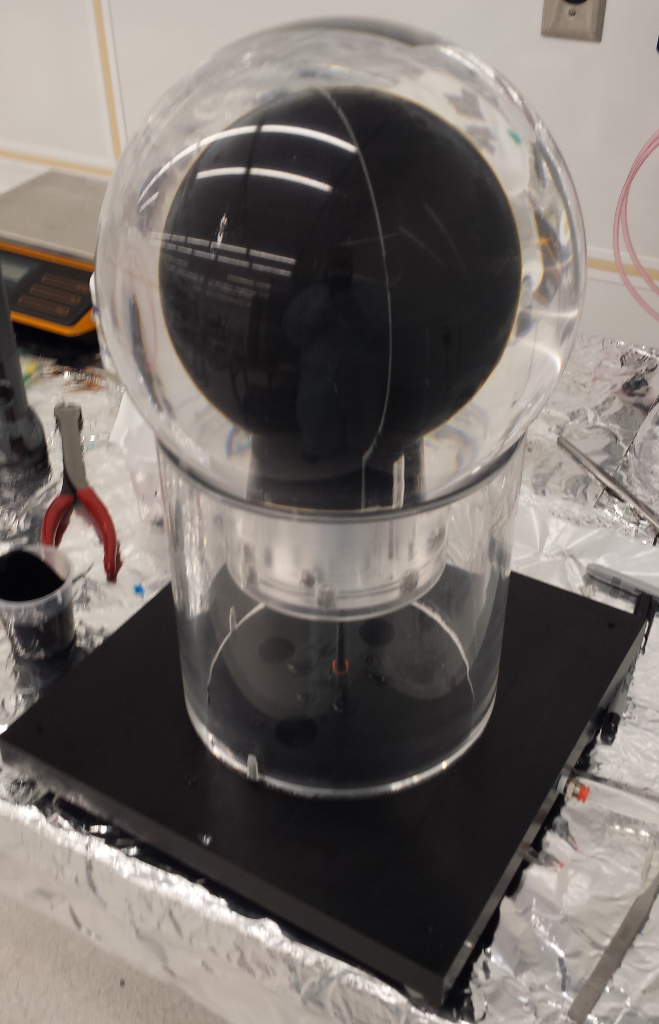
\includegraphics[width=\textwidth]{drying_stand.png}
  \caption{Test source drying on the drying stand.}
\end{subfigure}
\hspace{0.5cm}
\begin{subfigure}{.67\textwidth}
  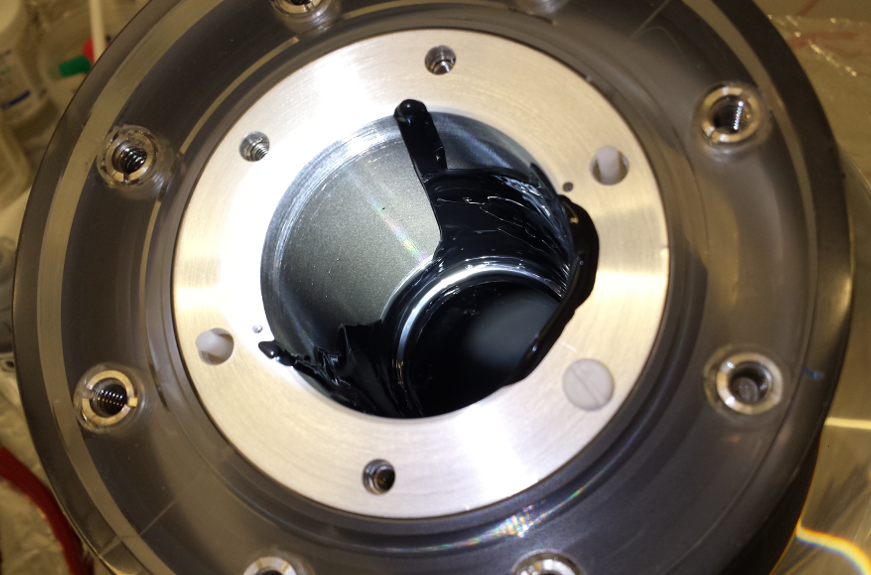
\includegraphics[width=\textwidth]{paint_drips.png}
  \caption{After drying the final black layer, the minimal excess paint dripping is cut away from the aluminum neck sleeve by a scalpel.}
\end{subfigure}
\caption{The painting and drying setup was tested with the test source in a class 1000 clean room at LBNL. Note that the neck sleeve used here for the test source was not anodized whereas the final source will have a black anodized aluminum neck sleeve.}
\label{fig:drying}
\end{figure}


For the first two of three opaque black layers a Teflon sleeve similar to the aluminum neck sleeve was inserted into the neck to prevent black paint from adhering to the neck region while allowing excess paint to drip out. Using a removable Teflon sleeve for the first two layers enhanced the uniformity of the paint thickness near the neck by preventing pooling (see Figure \ref{fig:minisource_paint}) that would occur if the aluminum neck sleeve were present. Prior to the third layer of black paint, the aluminum neck sleeve that accepts the PMT assembly was potted into the neck using Sylgard 184, a silicone encapsulate, allowing the third layer of black paint to fill any gaps around the neck sleeve to decay chamber interface resulting in a light tight seal. The encapsulate was applied to the outside of the neck sleeve and inserted into the source with the neck facing down to ensure no encapsulate dripped into the decay chamber. After the encapsulate cured on the drying stand, the final layer of black was applied.

The final layer was a mixture of 40\,mL of deionized water, 20\,mL of Vallejo white paint, and 5\,g of TPB. The addition of deionized water made the mixture approximately the same consistency as the black paint, and upon drying the remaining layer is mostly TPB crystals with a white paint binding that adheres well to the black paint surface. 5\,g of TPB using this deposition method was shown to give approximately the same scintillation brightness as the SNO \Li source when illuminated under a UV lamp.

\begin{figure}
\begin{subfigure}{.35\textwidth}
  \centering
  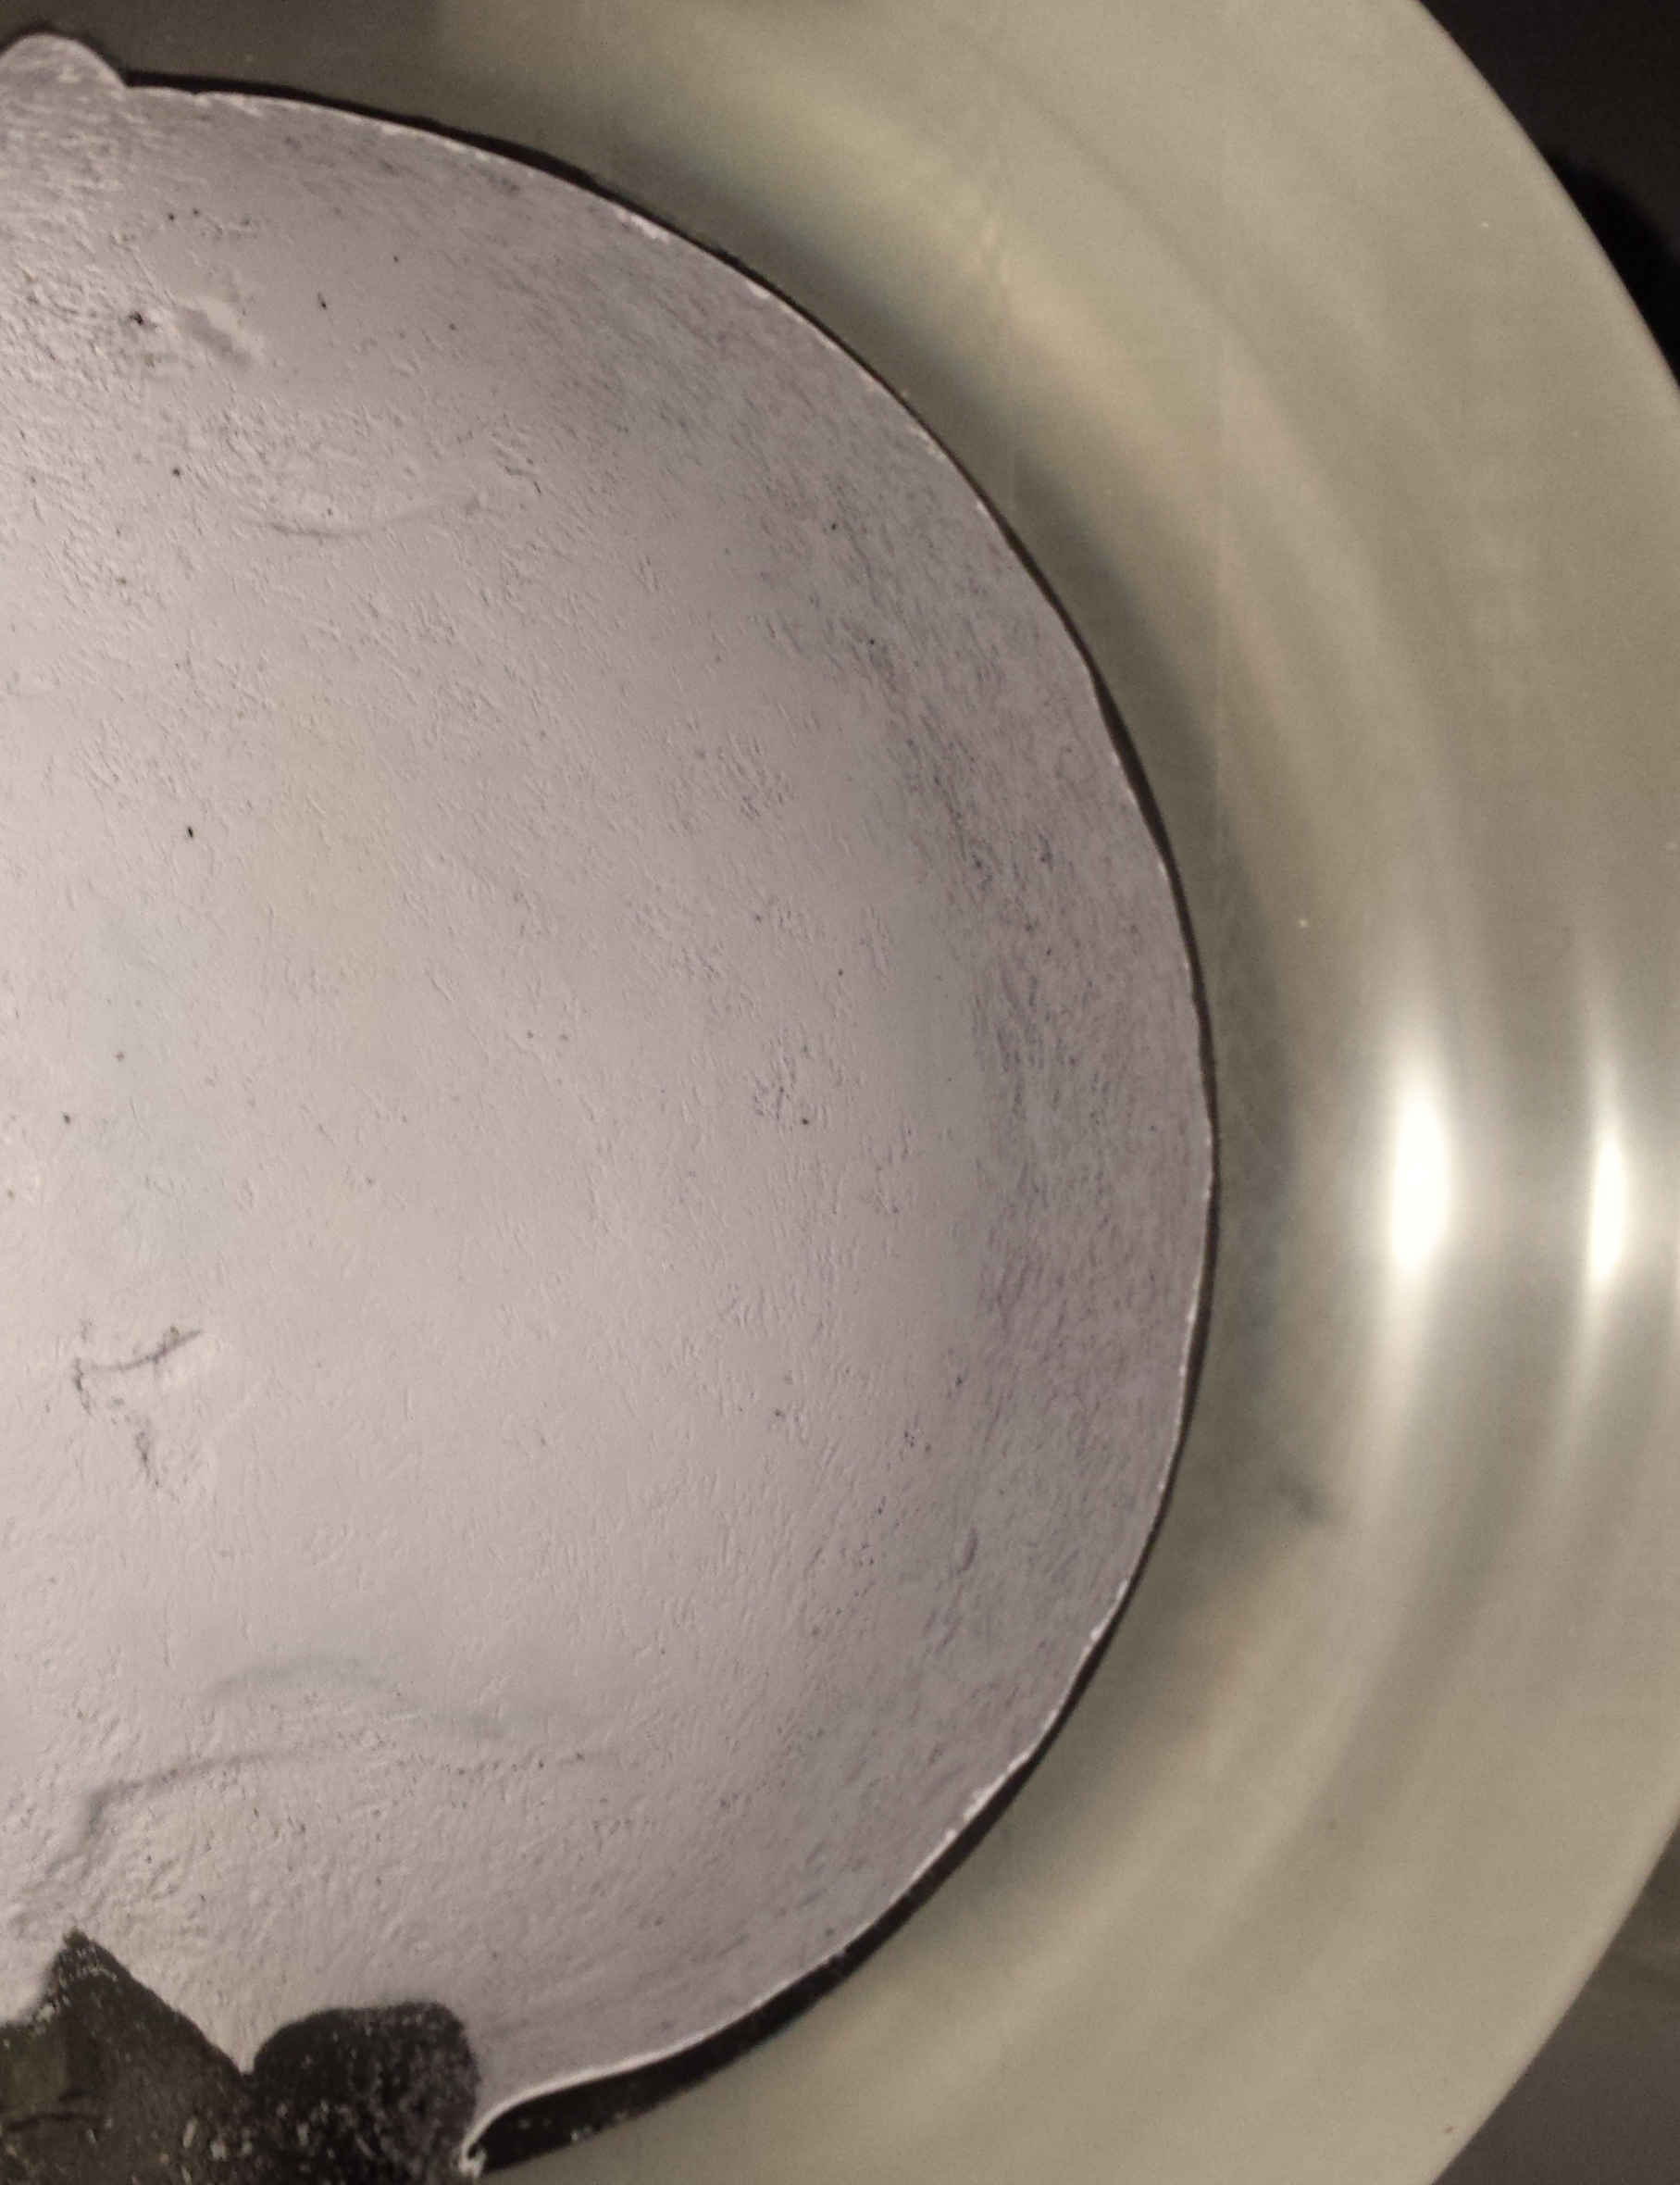
\includegraphics[width=0.8\textwidth]{minisource_paint.png}
  \caption{Small scale painting test showing cross-section of paint thickness. The pooling near the bottom was reduced by allowing easier drainage of paint for the first two layers, resulting in less anisotropy than pictured here.}
  \label{fig:minisource_paint}
\end{subfigure}
\hspace{0.5cm}
\begin{subfigure}{.55\textwidth}
  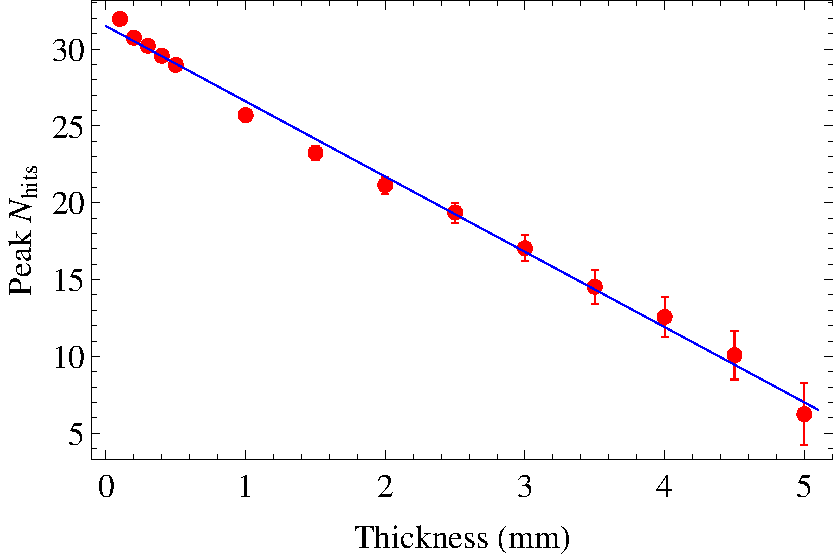
\includegraphics[width=\textwidth]{100k_realistic_nonoise_hits_vs_thickness}
  \caption{Simulation in scintillator phase SNO+ of \Li beta decays inside decay chamber volume with various smooth and isotropic paint layer thicknesses. As expected this follows a roughly linear trend representing the energy loss of the electrons in the paint.}
  \label{fig:meannhits}
\end{subfigure}
\caption{Small scale painting results and preliminary simulations of NHit response for \Li beta decays for various paint thicknesses assuming the simplest case of a smooth paint layer.}
\label{fig:prelimpaint}
\end{figure}

\subsubsection{Surface Quality and Thickness}

The mass of the source was measured before paint was added and after excess was cut away for each layer, which was used later to infer layer thickness. 
To ensure light tightness of the source, the gas inlet and outlet tubes were fitted with stainless steel capillaries that protrude into the decay chamber enough to allow the paint layers to form a light tight seal. 
To prevent these capillaries from filling with paint a Teflon rod is inserted that extends past the capillary into the decay chamber and remains for the entire painting process. 
The aluminum neck sleeve that receives the PMT and ensures light tightness of the neck region was added during the opaque paint layers.

After each layer the surface was visually inspected to ensure no major flaws or clumps were found. Smaller scale tests indicated that the paint layers will be thicker near the neck than opposite the neck due to the drying orientation (anisotropy), that the mean paint thickness would be around 1\,mm, and that 10\% variations in thickness (roughness) are to be expected (Figure~\ref{fig:minisource_paint}). The roughness is expected to vary with a characteristic length scale of approximately 1\,cm according to the cross section of the small scale paint test.

To explore the effects of mean thickness and surface roughness on NHits, simulations of \Li electrons were done using a source geometry in RAT and various different paint layers. Simulations with perfectly smooth paint layers indicated that a 0.1\,mm change in mean paint thickness is conservatively a 5\% change in mean NHits (Figure~\ref{fig:meannhits}), so it will be necessary to know the thickness of the paint very well. 

\begin{figure}[h!]
\begin{subfigure}{.53\textwidth}
  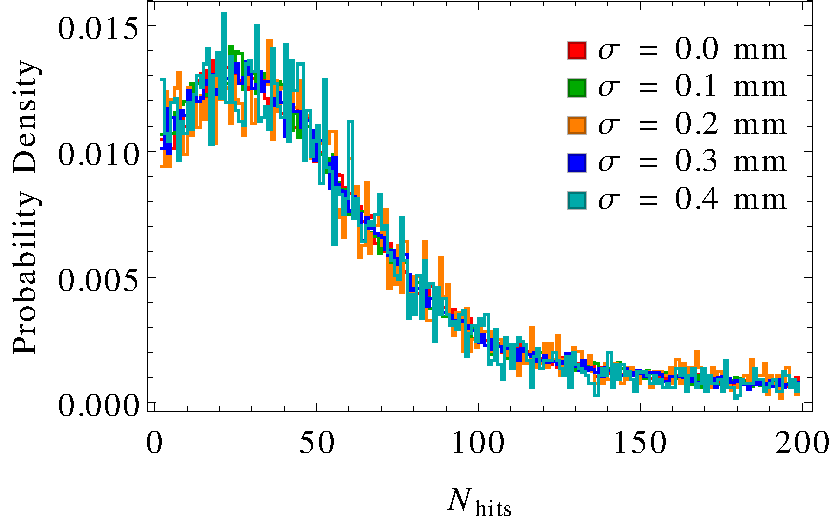
\includegraphics[width=\textwidth]{paint_uniformity_nhits_hists}
  \caption{Plot of NHit distributions for \Li beta decays inside a decay chamber with various paint surface roughnesses. The sigma value here is roughly the standard deviation of the fluctuations in thickness, which were generated with a feature size of 1\,cm. The 0.2\,mm and 0.4\,mm plots have 10x fewer statistics due to simulation difficulties.}
  \label{fig:simulations}
\end{subfigure}
\hspace{0.5cm}
\begin{subfigure}{.38\textwidth}
  \centering
  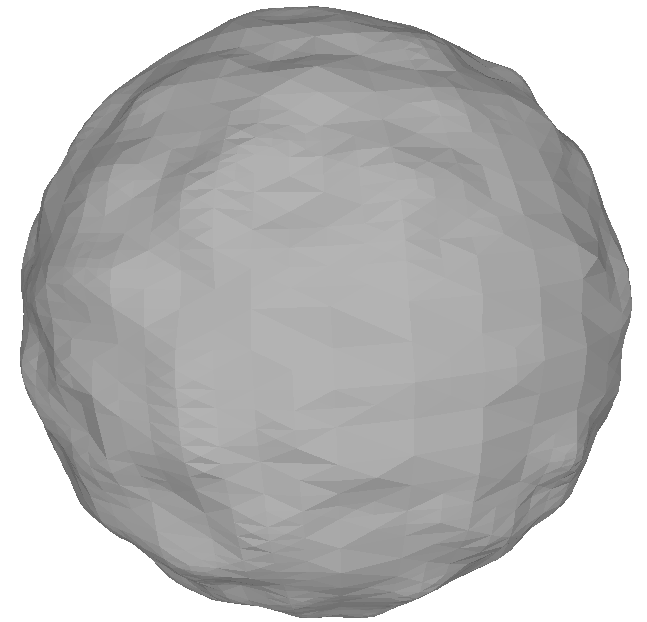
\includegraphics[width=0.85\textwidth]{0p5mm.png}
  \caption{Rendering of an STL defined paint surface imported into GEANT4 using perlin noise to simulate the expected roughness of the surface based on small scale tests. This is a sigma of 0.5~mm, which exaggerates the roughness enough to be clearly visible.}
  \label{fig:rough_sphere}
\end{subfigure}
\caption{Simulations with STL defined surfaces taking roughness and anisotropy in the paint layer into account show that neither has a strong effect on the NHit distributions.}
\label{fig:stltests}
\end{figure}

By generating stereolithography (STL) surface definitions, which break an arbitrary surface down into triangles, and importing these into RAT/GEANT4, it was possible to simulate how paint roughness or anisotropy would change the peak NHits. 
Figure~\ref{fig:stltests} summarizes the result that the expected roughness and anisotropy had no significant effect on the mean NHit. 
Since events are uniform in the decay chamber volume, and hence any individual beta sees a distribution of thicknesses of paint based on initial position and direction regardless of surface imperfections, the fact that these effects do not contribute strongly makes sense. 
Therefore it was only necessary to establish the mean paint thickness accurately to properly simulate the NHits distribution.

\begin{figure}[h!]
\begin{subfigure}{.45\textwidth}
  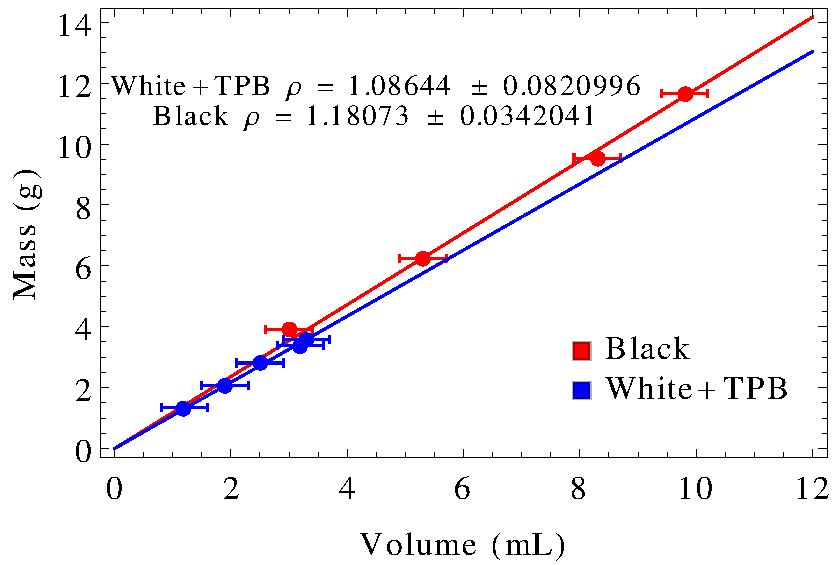
\includegraphics[width=\textwidth]{paint_density}
  \caption{Summary of density fit for black and white+TPB paint layers. The uncertainty on the mass of the samples was insignificant, and therefore the largest source of error was the volume measurement, which was done with water displacement in a graduated cylinder with 0.2\,mL divisions and a tolerance of 0.2\,mL.}
  \label{fig:paintdensity}
\end{subfigure}
\hspace{0.5cm}
\begin{subfigure}{.45\textwidth}
  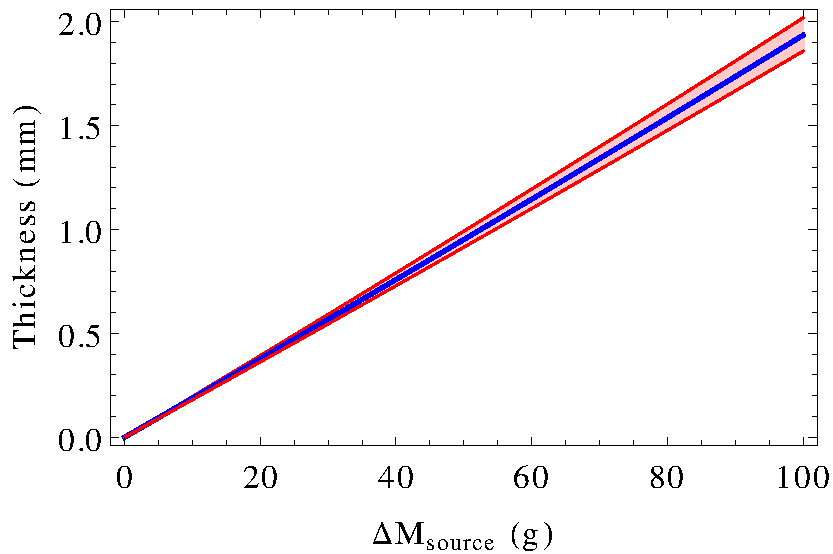
\includegraphics[width=\textwidth]{paint_rough_thickness}
  \caption{Assuming a simple uniform coverage model in the geometry of the source, this shows the mean and uncertainty on a thickness prediction for black paint given a measured change in the mass of the source. This can be further refined by taking into account non-uniform coverage. }
  \label{fig:paintthickness}
\end{subfigure}
\caption{Paint density data used in the weight to thickness conversion and a preliminary estimate of how well the calculation will work.}
\label{fig:weightmeasure}
\end{figure}

Many options for directly measuring the paint layer thickness were explored and ultimately rejected based on cost or lack of required precision. The final decision was to infer the paint thickness from the change in mass of the source before and after painting each layer. With a total source weight of 8.2\,kg and an expected total paint weight of 50\,g this required a scale capable of weighing 0.1\,g on top of 10\,kg so that uncertainty in weight was not a dominant source of error. The densities of the dry paint used in the black and white layers were fit using volume and mass measurements of small dry samples. These density results are summarized in Figure~\ref{fig:paintdensity}, and errors on these densities were the dominate sources of error for the thickness calculation. 

Figure~\ref{fig:paintthickness} gives a rough projection of estimated paint thickness for a given change in source mass. To do this conversion the change in mass must be converted to a paint volume, and the volume must be converted into a thickness using some model for how the paint coats the surface of the decay chamber. Using the source designs a model of paint coverage was developed as described in Figure~\ref{fig:surfacemodel}, which ignores surface roughness since this should average out to the mean thickness. Based on small scale tests the expected anisotropy should lead to the neck area being roughly twice as thick as the thinnest section opposite the neck, however, according to this model an uncertainty in anisotropy does not significantly change the inferred mean thickness. Ultimately this measurement procedure for the test source led to an inferred thickness of $1.02\pm0.04$\,mm, or approximately a 4\% uncertainty on the peak NHits.

\begin{figure}[h!]
\centering
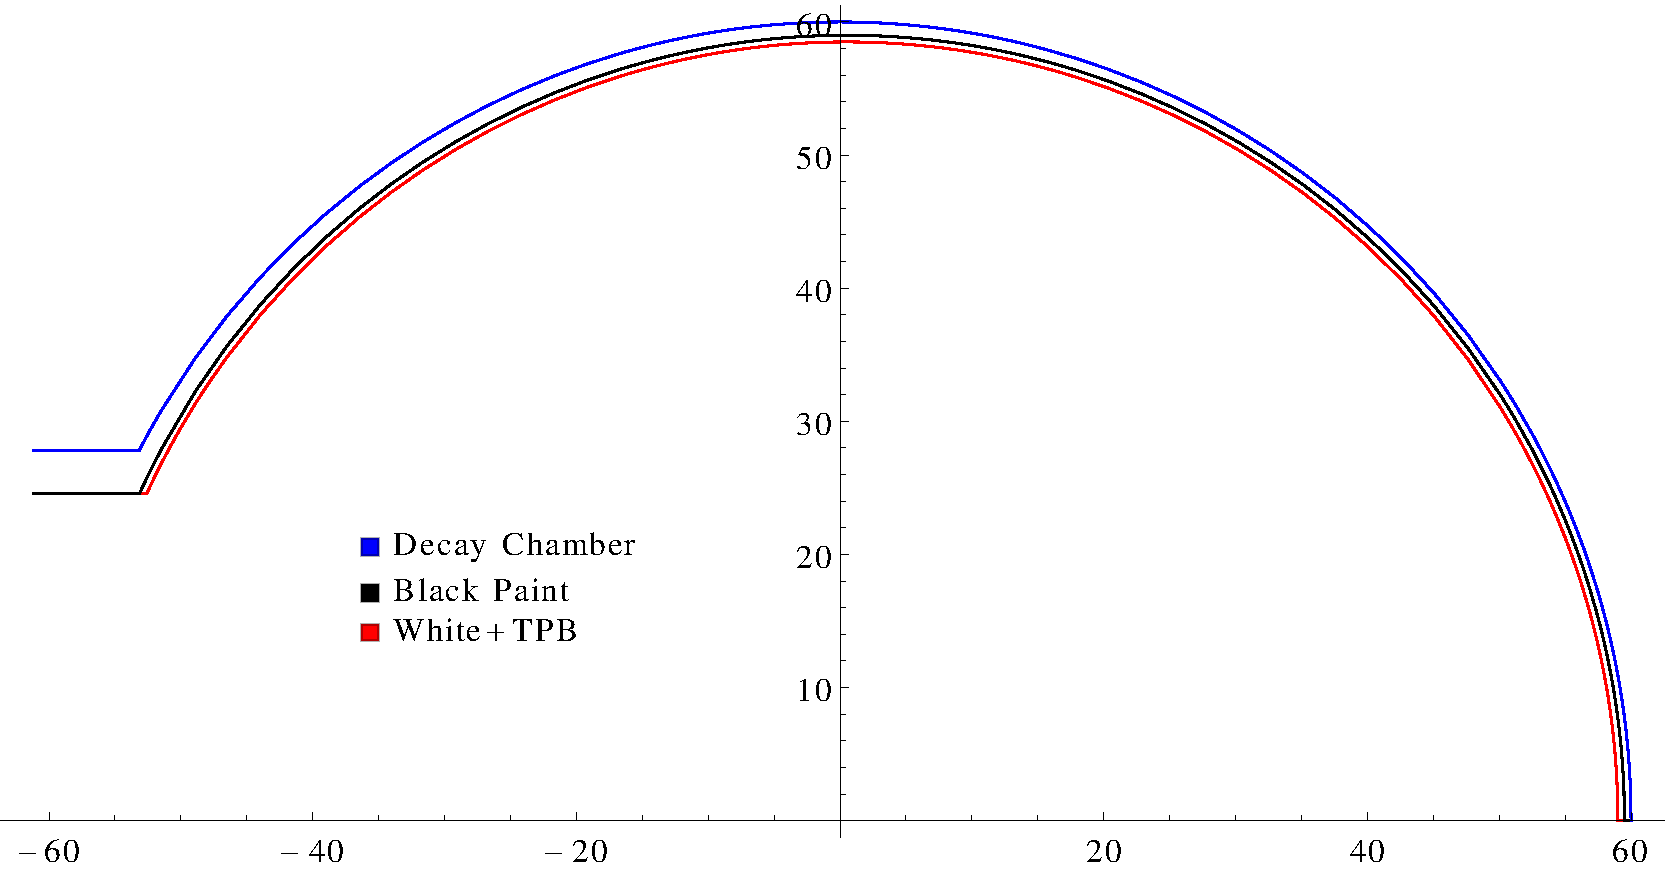
\includegraphics[width=0.7\textwidth]{paint_model}
\caption{The cylindrical profile of the full coverage model is shown here. This was revolved numerically to calculate the volume and hence the mass of the paint for a particular set of parameters to get a mass to thickness lookup table. Anisotropy in the paint thickness is accounted for by offsetting the inner surface of the black paint layer by some amount. In small scale tests this offset was empirically approximately half the mean thickness of the paint, and using this model it was verified that uncertainty in this anisotropy contributed a negligible uncertainty to the estimated mean thickness. The parameters for this profile are a black thickness of 1.0\,mm, anisotropy offset of 0.5\,mm, and white thickness of 0.5\,mm. }
\label{fig:surfacemodel}
\end{figure}

\subsection{PMT assembly potting}
The PMT used for the source is the Hamamatsu H11432-100, which has an integrated high voltage supply that requires only low voltage (+5V) to operate. This is advantageous because there will be helium gas inside the source, which would form a plasma if exposed to high voltage, and this configuration does not require providing high voltage via the umbilical. However, the PMT supply itself does not come potted and helium gas could leak inside resulting in a plasma that would damage the PMT and possibly the source. To prevent this the high voltage supply module was potted into an anodized aluminum potting sleeve with Sylgard~184, a silicone encapsulate, which was also allowed to fill the cavity containing the supply and around the body of the PMT as shown in Figure~\ref{fig:potting}. To ensure the encapsulate fully filled the cavities the assembly was placed in a soft vacuum between applications of encapsulate to assist in removing air that may have been trapped. This entire potted PMT assembly fits directly into the neck sleeve and contains the o-rings that isolate the decay chamber from the rest of the source, so this potting serves the additional purpose of making the PMT assembly into a solid part to isolate the decay chamber from the rest of the source. 

\begin{figure}
\begin{subfigure}{.385\textwidth}
  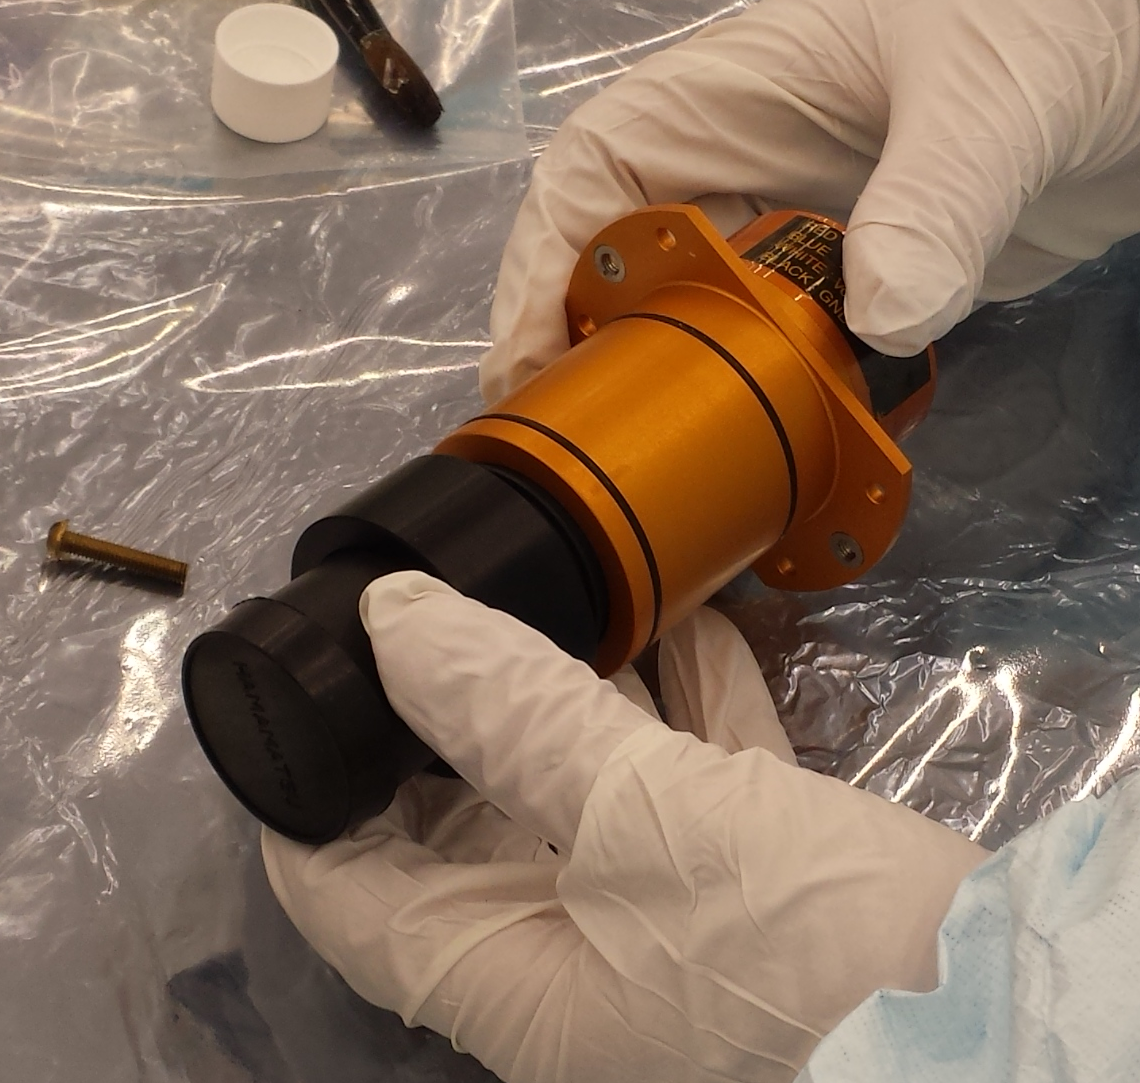
\includegraphics[width=\textwidth]{potting_1.png}
  \caption{The PMT to be potted inside the anodized aluminum spacer (black) and anodized aluminum potting sleeve (orange).}
  \label{fig:potting_a}
\end{subfigure}
\begin{subfigure}{.305\textwidth}
  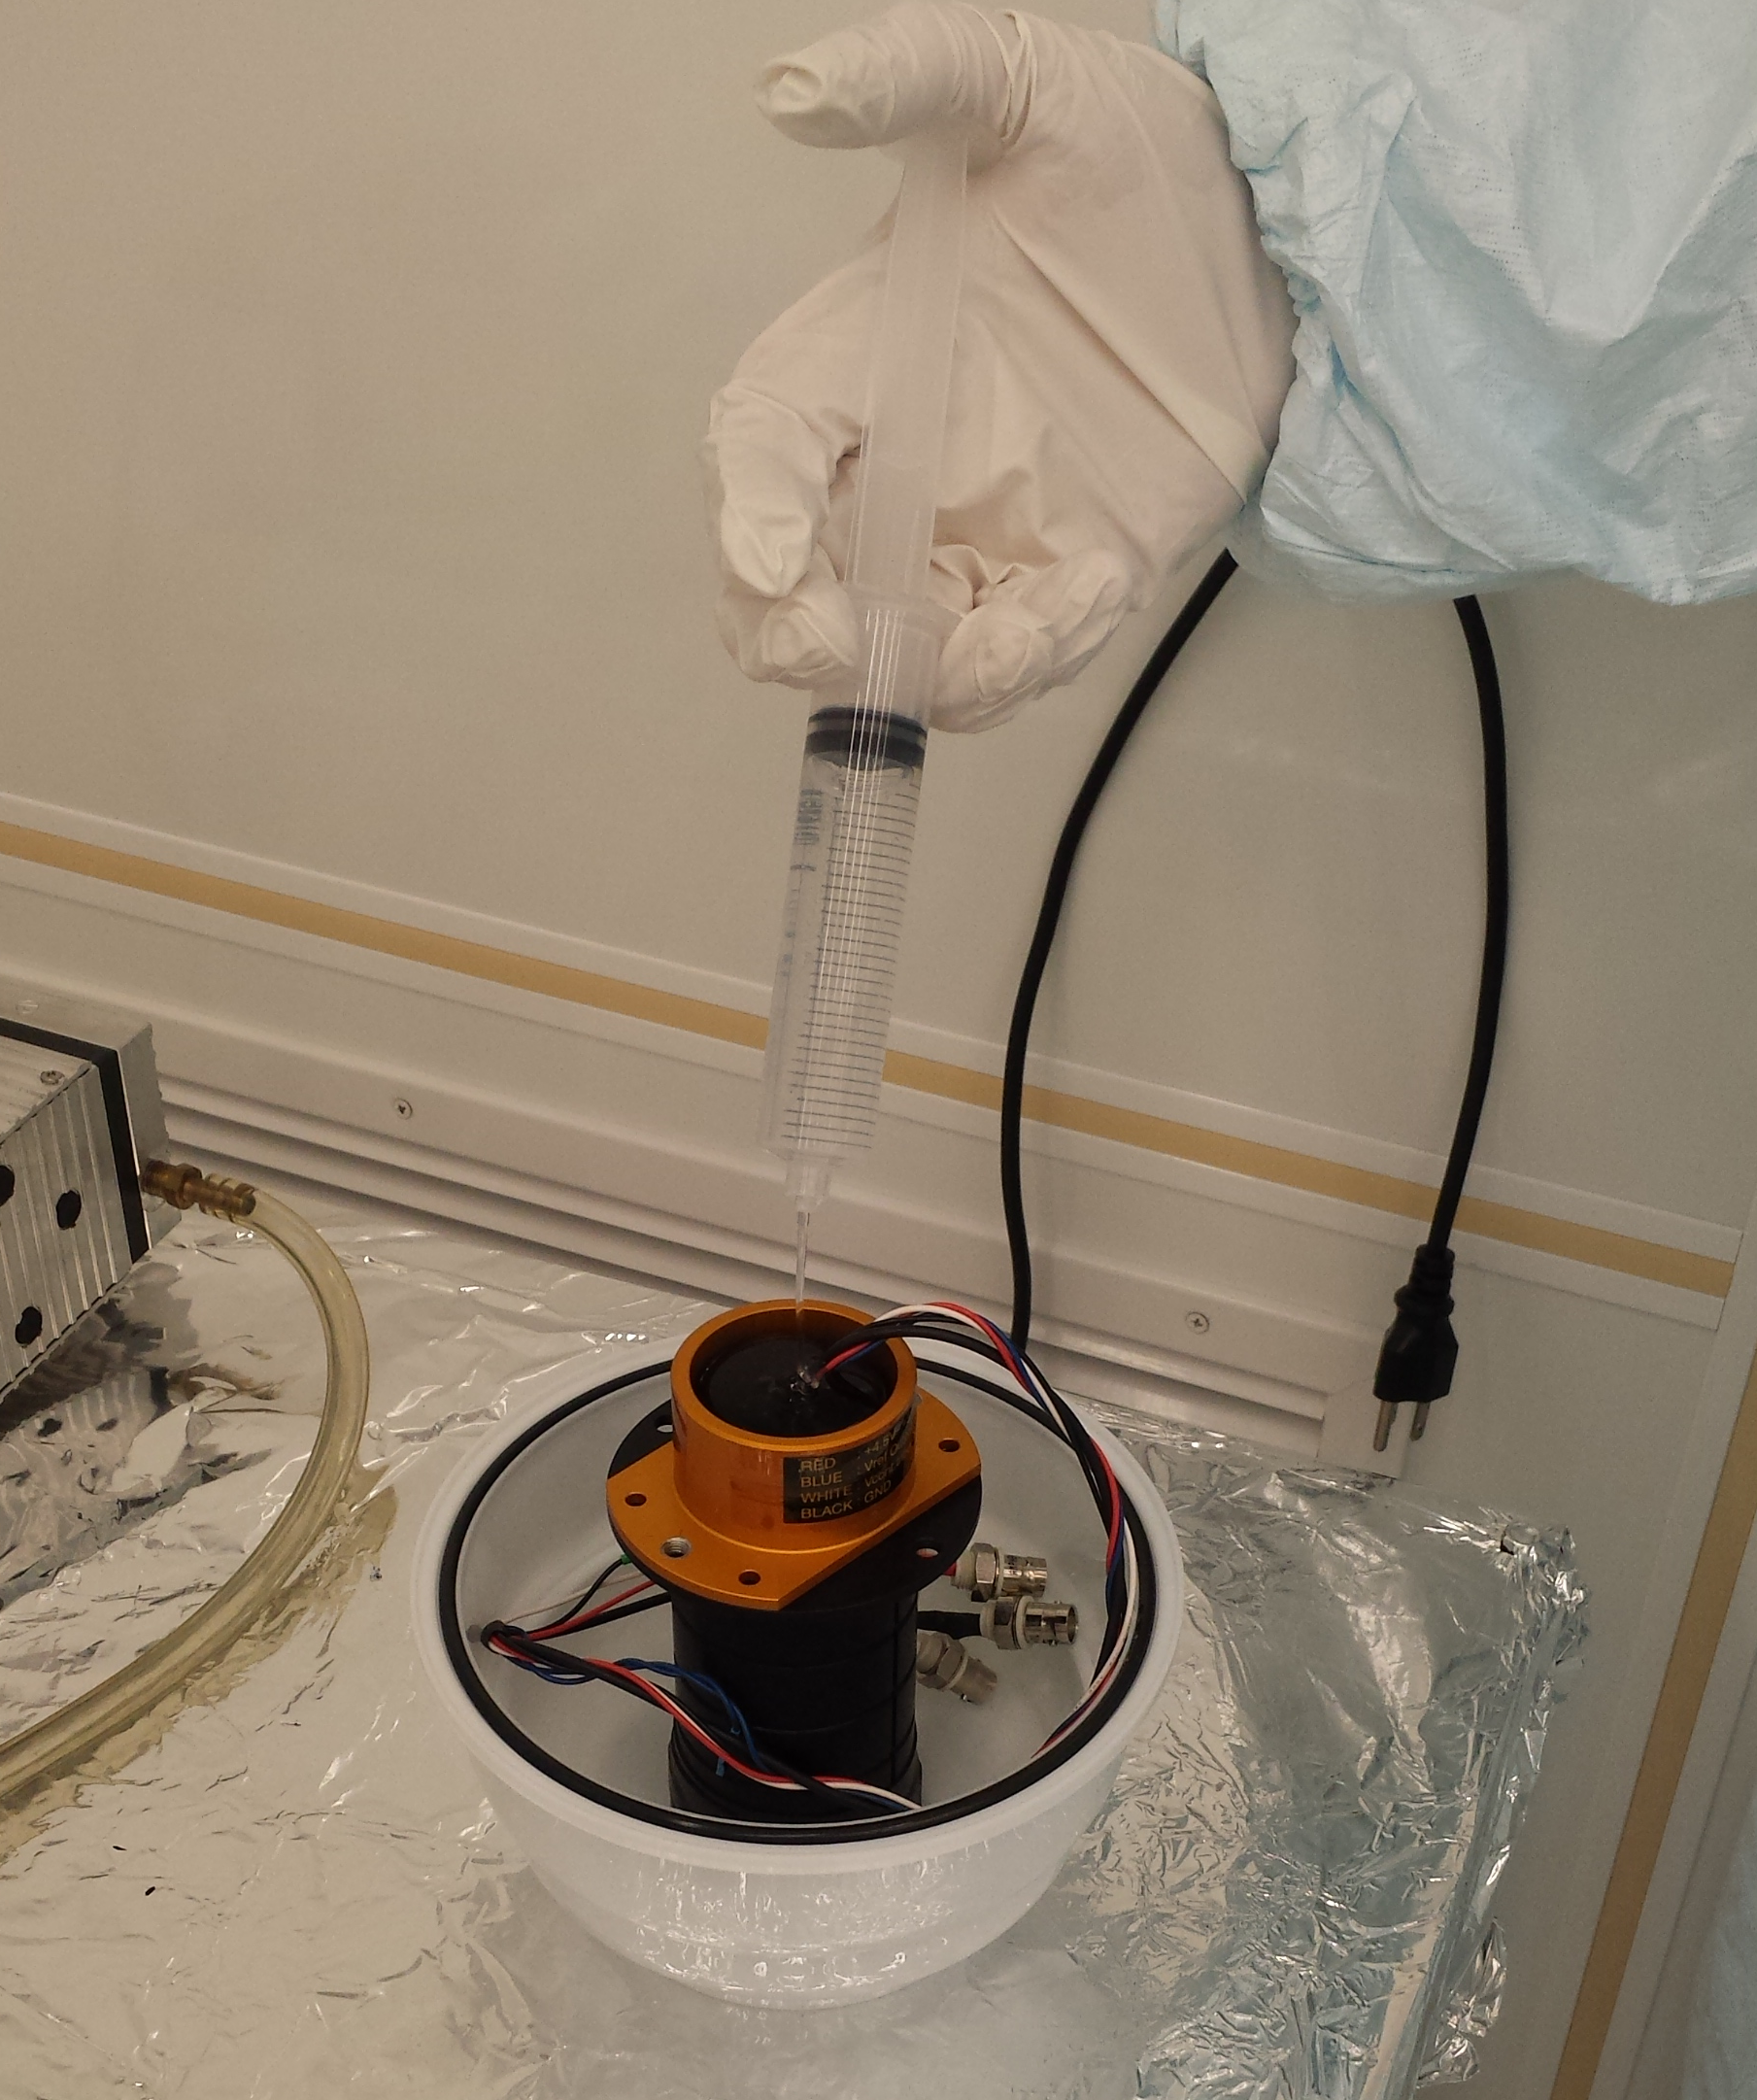
\includegraphics[width=\textwidth]{potting_2.png}
  \caption{Encapsulate added in stages with vacuum between to fill areas with trapped air}
  \label{fig:potting_b}
\end{subfigure}
\begin{subfigure}{.29\textwidth}
  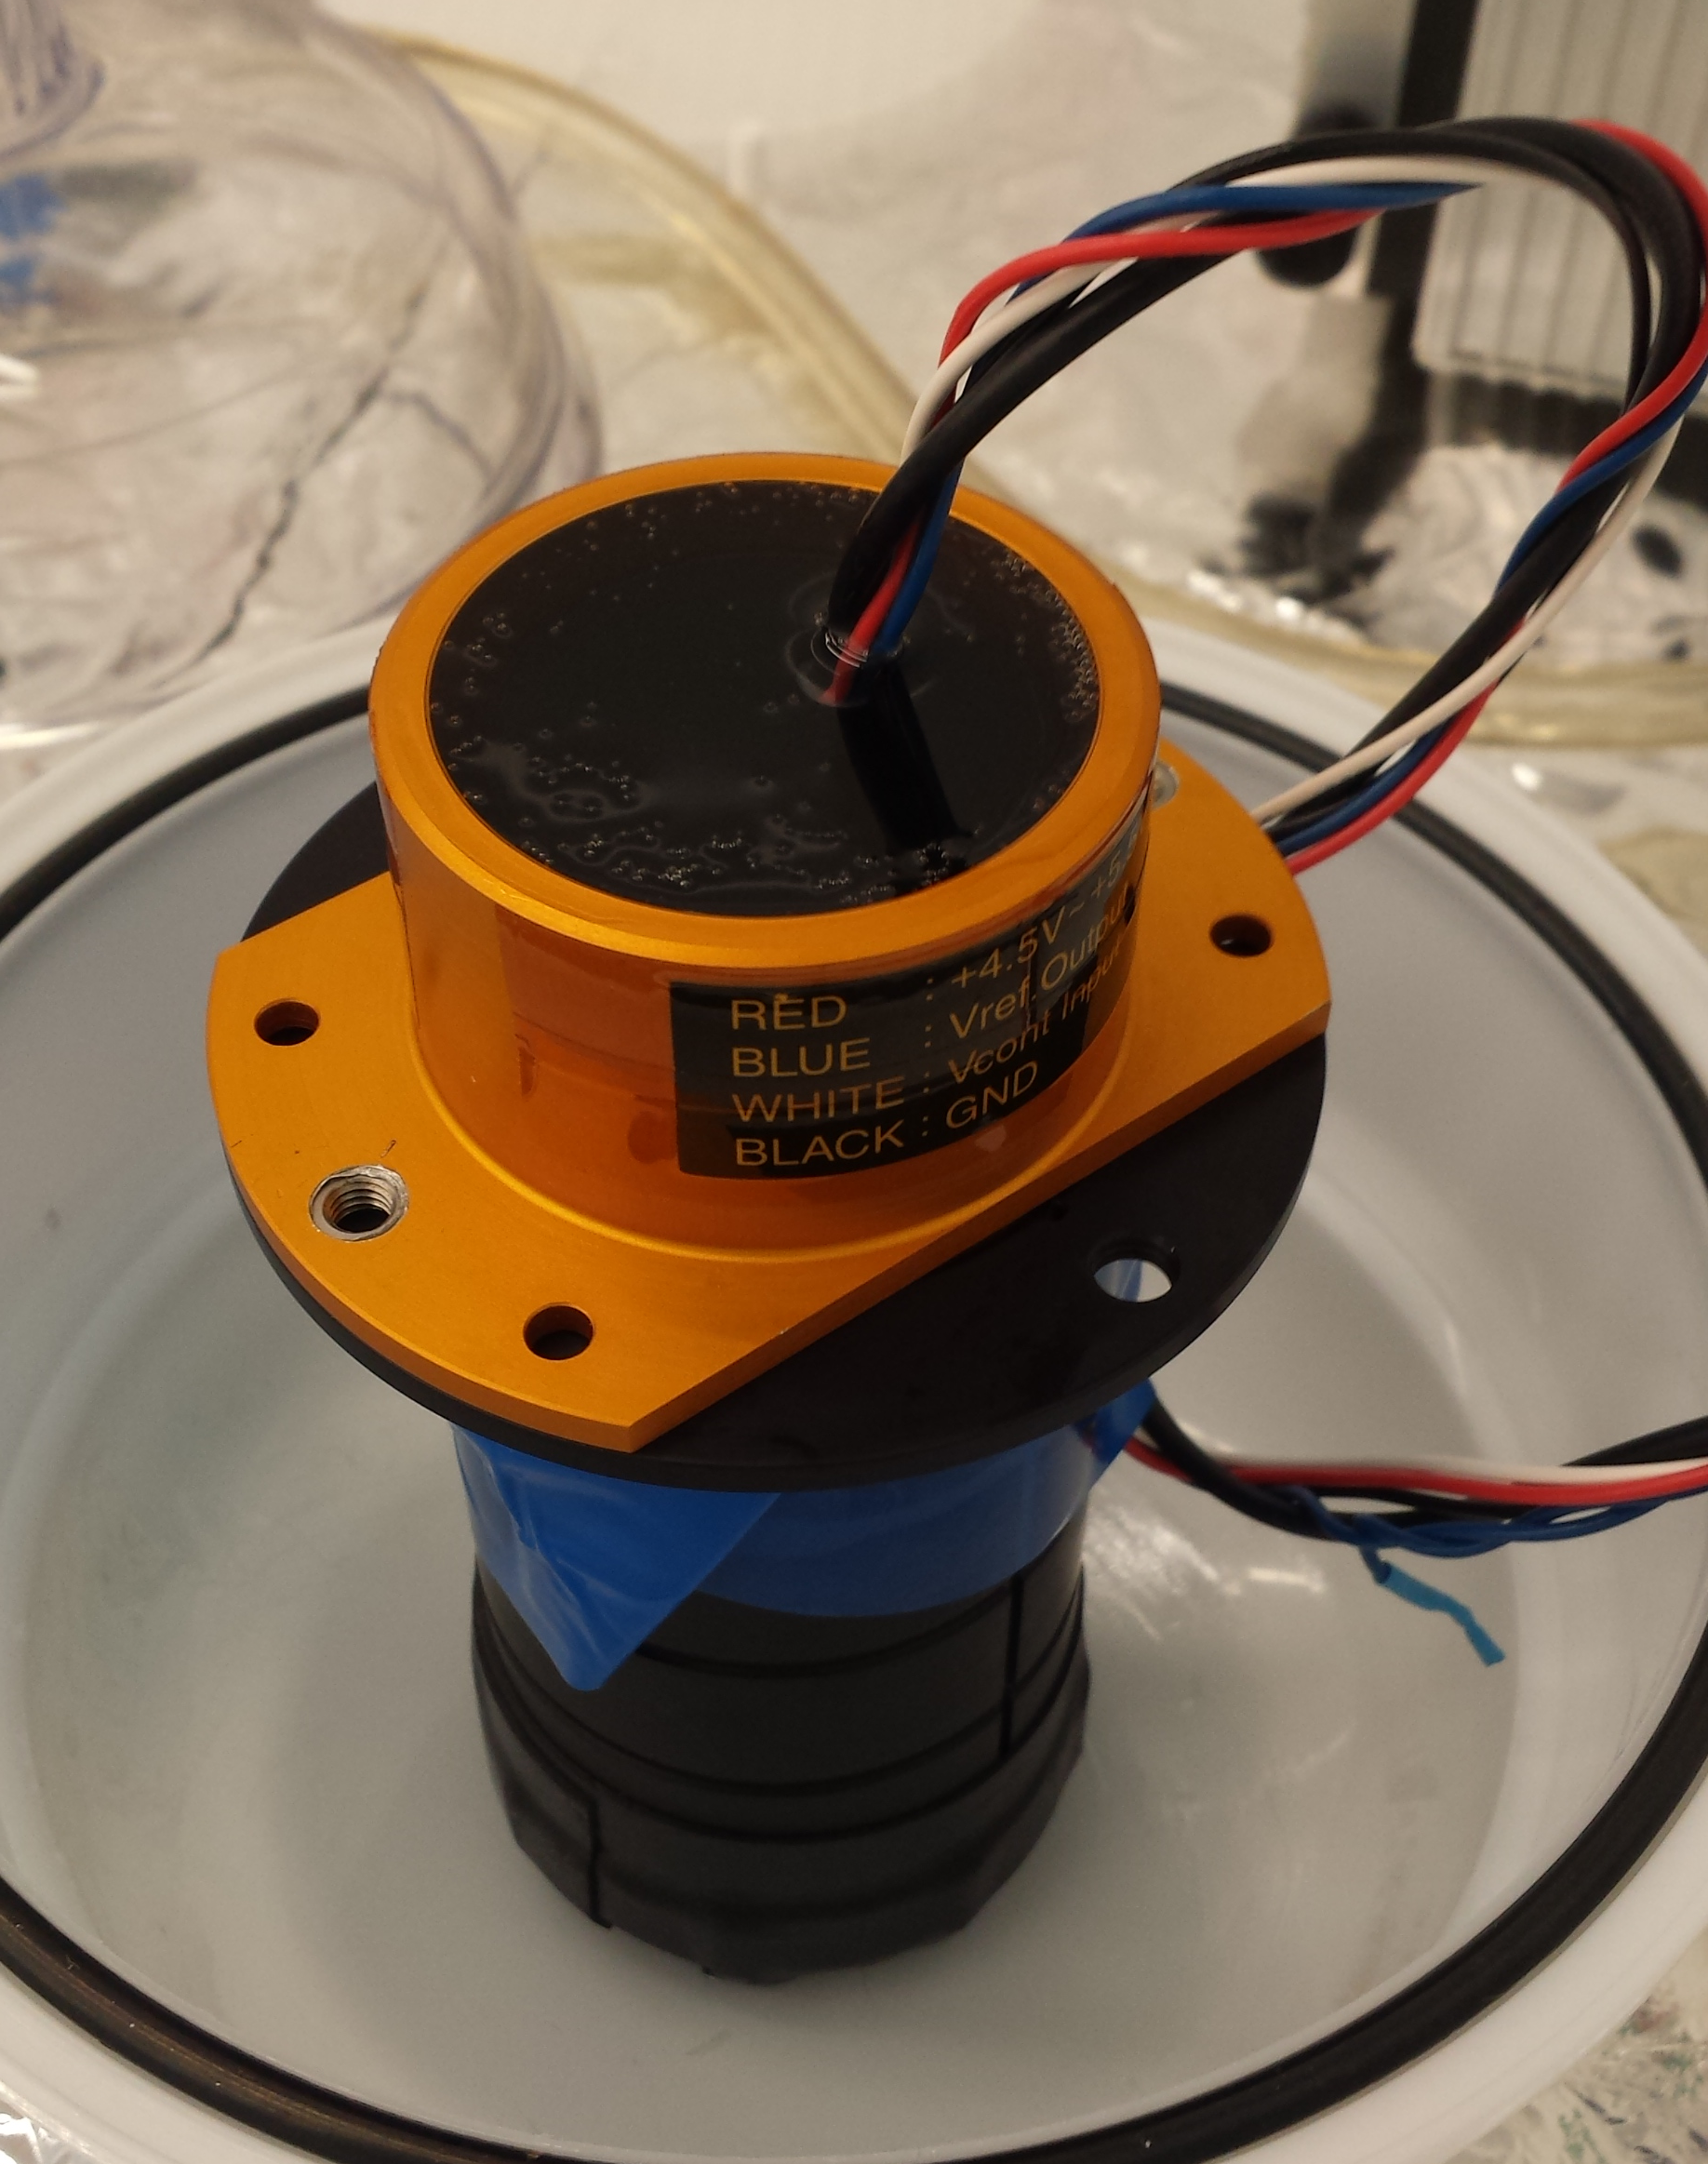
\includegraphics[width=\textwidth]{potting_3.png}
  \caption{Finally the encapsulate was allowed to cure in the clean room.}
  \label{fig:potting_c}
\end{subfigure}
\caption{Potting of the PMT into the anodized aluminum components for the final source. All work was done in the class-1000 clean room at LBNL.}
\label{fig:potting}
\end{figure}

\section{Source Quality Control}
\label{chap:tests}

This section describes the tests that were done on the source and the source materials to verify that the construction met the background and safety requirements for SNO+. 
Of concern here are any radioactive contamination that may be present in the source materials and any adverse affect the source materials may have on the target medium of the detector.
Since the source is primarily acrylic and stainless steel, no radioactivity or material compatibility concerns are expected, but the potential impact of catastrophic failure of the source (target material entering the decay chamber and flowing back into the detector) must be evaluated.

\subsection{Radon Emanation Estimate}
\label{sec:emanation}
The decay of radon is part of the thorium and uranium decay chains, and its decay produces many radioactive daughter nuclei that are important radioactive backgrounds.
Radon itself is a particular issue because it is a gas at room temperature, and can readily move from one material to another.
It is therefore important to constrain the amount of radon expected to emanate from a calibration source, because this radon will increase the radioactive backgrounds within the detector.
A first pass radon emanation estimate can be calculated by considering the surface area of stainless steel and acrylic that will be exposed during deployment. 
Estimates for the radon emanation of the UI used a measurement of $4.60$ $\mu$Bq m$^{-2}$ for stainless steel \cite{kormos:2015}. 
The SNO stainless steel limit was $< 5$ mBq m$^{-2}$ and for acrylic $< 1.6$ mBq m$^{-2}$ \cite{Liu:1993}. 
The source, assuming a full size stainless steel housing, has an exposed stainless steel surface area of $0.15$ m$^2$, and exposed acrylic surface area of 0.20 m$^2$. 
Assuming the stainless steel housing remains at its full size and can reach the cleanliness standards assumed in the UI emanation estimate, this leads to a total radon emanation from the exposed surfaces of the source to $<28$ atoms/day where this limit is grossly dominated by the limit on the acrylic radon emanation. 
The radon emanation rate for stainless steel is, however, significantly lower in the source used by the UI document than number used by SNO, which either means the UI estimation is unrealistic or the SNO limit was very conservative. 
Using the limits from the SNO measurements we would expect $<92.5$ atoms/day.
In either case, this is expected to be within the as-yet undefined SNO+ radon budget for scintillator phase.

\subsection{Intrinsic Radioactivity}
\label{sec:matcounting}
All materials have some level of radioactive contamination from natural sources.
In most cases this intrinsic radioactivity is at such low levels that it can be safely disregarded, however, being present in the target volume of a neutrino detector is not one of those cases.
In fact, deployment in SNO+ will be the best measurement of the radioactivity of this source, but other methods must be used prior to deployment to place limits on such radioactivity and ensure there is not unexpected contamination.
This is done in two ways: source materials can either be placed in low background radiation detectors and directly measured, or the materials may be exposed to a high neutron flux, which activates the trace materials in the source making them easier to measure.
As this source is not expected to have radioactive contamination at detectable levels, direct measurement is not particularly useful, however, this was done for the acrylic at the Low Background Counting Facility at LBNL.
The neutron activation analysis (NAA) results were obtained by deployment of materials at the McClellan Nuclear Research Center and counted at UC Davis. 
See Table \ref{tab:counting} for counting results for materials used in the source.

\begin{table}[h!]
\centering
\begin{tabular}{|l|l|l|l|l|l|} \hline
                    Material       & Mass & Method    & $^{238}$U     & $^{232}$Th    & $^{40}$K      \\ \hline
 \multirow{2}{*}{UVA acrylic}  & 8096.7\,g & NAA    & $<$81\,ppb    & $<$24\,ppb   & $<$2.1\,ppb   \\ \cline{3-6}
                                   & & Direct & $<$0.8\,ppb &$<$0.8\,ppb & $<$0.4\,ppm \\ \hline
                    Black paint    & $\approx 50$\,g & NAA    & $<$252\,ppb   & $<$37\,ppb   & $<$3.9\,ppb           \\ \hline
                    TiO paint      & $\approx 1.5$\,g & NAA    & $<$2.8\,ppm   & $<$189\,ppb  & $111.5 \pm 8.6$\,ppb           \\ \hline
                    TPB            & $\approx 4$\,g & NAA    & $<$0.8\,ppm   & $<$237\,ppb   & $<$47.1\,ppb  \\ \hline
                    Sylgard silicon& $\approx 200$\,g & NAA    & $<$116\,ppb   & $<$48\,ppb   &6.7$\pm$1.5\,ppb\\ \hline
\end{tabular}
\caption{\label{tab:counting} Cherenkov source material counting results. Approximate masses are estimates from the test source that should be approximately the same for the final source upon its completion.}
\end{table}

Out of all the materials, only the potassium levels in the TiO white paint and the Sylgard silicon resulted in measurements instead of limits. 
All the other measurements yielded upper limits meaning the signal was below the measurement sensitivity of the method. 
Except for the UVA acrylic, none of the tested materials are expected to come into contact with the target material, and the lack of a detectable radioactive signal here definitely meets the requirements for deployment.
Detectable potassium levels from NAA in the materials within the source are not expected to be an issue because the total amount of material present within the detector is small, and the target material should not come in contact with these materials in normal operation.

\subsection{Material compatibility tests}
\label{sec:comptest}
Beyond basic concerns of chemical compatibility, the light yield and optical properties of the LAB+PPO scintillator used in SNO+ are quite dependent on the exact chemical makeup of the scintillator.
Additionally, the scintillator itself is a solvent, so there is a very real possibility that a material immersed in LAB+PPO could leech into the scintillator resulting in undesirable optical effects.
As such, any material expected to come into contact with LAB+PPO must first be exposed to it in some controlled way while the optical properties of the scintillator are monitored.
Further, materials that could possibly come in contact with LAB+PPO must not cause undesired chemical reactions if they are accidentally exposed.
Both UVA acrylic and stainless steel have been vetted by SNO+ (the AV is acrylic, and the process system for LAB+PPO purification is stainless steel), however, other Cherenkov source materials were vetted.

Three samples were tested for compatibility with LAB-PPO by the technical support team at SNOLAB: the potting material (Sylgard~184), a UVA acrylic sample with black paint and one with both black and white paint, and TPB mixed. 
These represent the materials inside the decay chamber that could potentially be exposed to LAB+PPO in the event of a catastrophic source failure.
The materials were soaked in a few 100\,mL of 2g/L PPO-LAB for 1 month. 
A control sample consisting of the default 2g/L PPO-LAB was scanned with the samples and used as a comparison. 
Deviation from the control is observed in all of the samples indicating incompatibility, however, no chemical reactions were observed.
Since these materials are not expected to come in contact with the LAB+PPO and are only present in small quantities within the source, this was deemed acceptable.
For the full technical report of the compatibility test, see~\cite{lina:2015}.


\subsection{Decay Chamber Opacity}
\label{sec:liningtest}
The light tightness of the decay chamber lining was validated on the full scale test source. 
To do this, the test source was placed in a dark-box with the center of the source 12" away from a 10" Hamamatsu R7081 HQE PMT, which has the SPE peak clearly separated from the noise. 
\begin{figure}
        \begin{subfigure}{0.49\textwidth}
                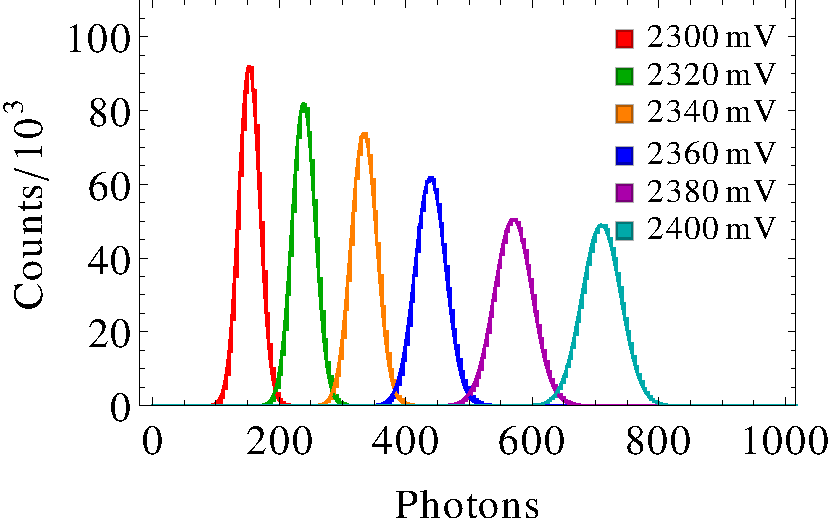
\includegraphics[width=\textwidth]{led_calibration_raw}
                \caption{Raw detected photon data at various voltages.}
                \label{fig:ledRAW}
        \end{subfigure}%
        \hspace{0.2cm}
        \begin{subfigure}{0.49\textwidth}
                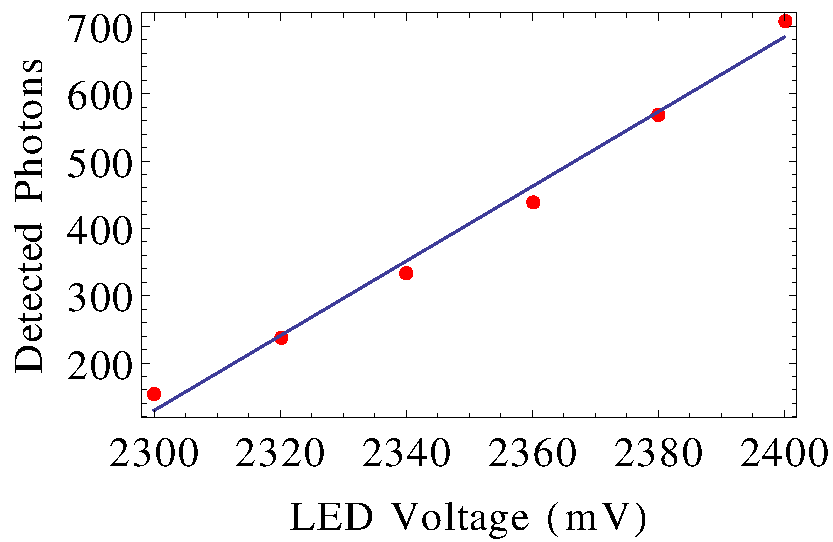
\includegraphics[width=\textwidth]{led_calibration_fit}
                \caption{Fit to the peaks of the photon distributions plotted against pulse voltage.}
                \label{fig:ledFit}
        \end{subfigure}
        \caption{Calibration data for the LED used to test the light tightness of the decay chamber lining. LED intensity was measured at 50\,cm from a R7081 10" PMT. The LED was pulsed at 50\,ns at various voltages.}
\label{fig:calibratedled1}
\end{figure}

A calibrated LED (see Figure \ref{fig:calibratedled1}) around the emission wavelength of TPB was placed in the center of the source with the neck blocked by an opaque rubber plug. This LED was pulsed on for 50\,ns intervals at various voltages one million times per LED voltage setting. The signal from the PMT was digitized and integrated with a per event pedestal correction to obtain a signal charge distribution. To cancel out systematics, the same process was repeated with the LED off to obtain a background charge distribution. The leaked light charge distribution was obtained by subtracting the background charge distribution from the signal charge distribution. There were no samples in the background subtracted charge distribution that appeared to correspond to multi-photon events, so each event that registered charge in the leaked light charge distribution was counted as a single leaked photon. The sum of leaked photons for the million events at each voltage are shown in Figure \ref{fig:lightleak}. 
\begin{figure}
        \begin{subfigure}{0.47\textwidth}
                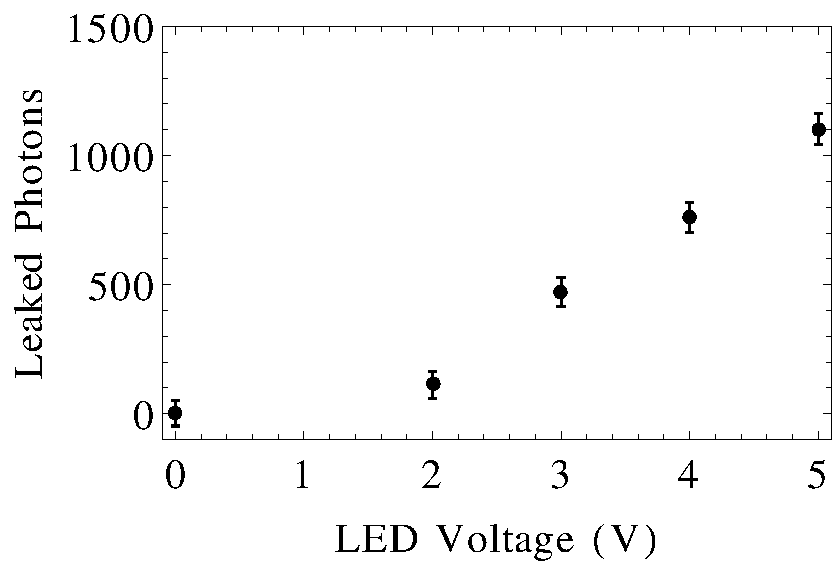
\includegraphics[width=\textwidth]{leakedphotons}
                \caption{Raw data showing the total number of photons detected by the PMT at the different led voltages tested where each datapoint is the sum of 1,000,000 events. Note the expected linear trend after the LED turns on around 2V. The uncertainties here are statistical measurement error.}
                \label{fig:lightleak}
        \end{subfigure}%
         \hspace{0.2cm}
        \begin{subfigure}{0.49\textwidth}
                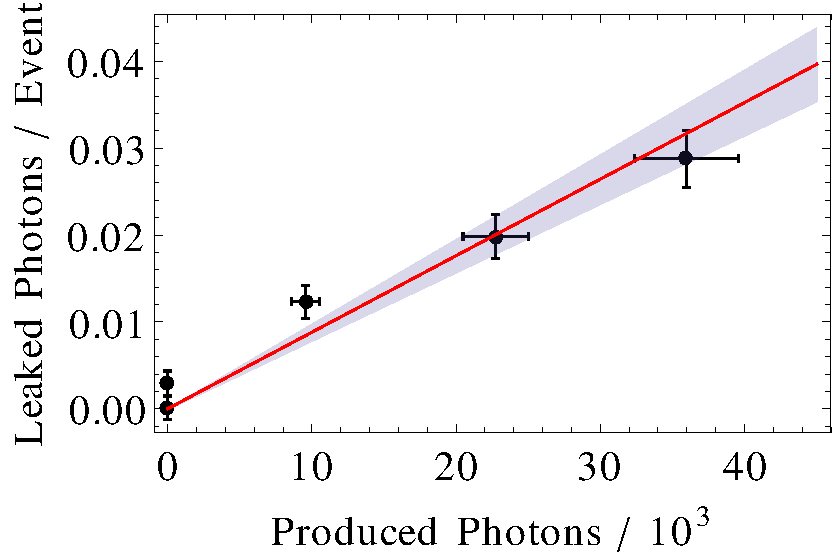
\includegraphics[width=\textwidth]{light_leak}
                \caption{Data showing the expected number of photons to leak per event from the source given some number of thousands of photons produced per event in the source.}
                \label{fig:eventleak}
        \end{subfigure}
        \caption{Summary of the data collected on the light tightness of the decay chamber lining. The actual expected light leak is, conservatively, on the order of 1 photons in 50 events.}
\label{fig:calibratedled2}
\end{figure}

To determine the total light leak of the source assume that the light leaking from the source is isotropic such that the PMT sees only a fraction of the total $4\pi$ light leak. Since the LED inside the source was pointed directly at the PMT, this is a conservative assumption. This along with dividing by the total number of events converts the y-axis of Figure \ref{fig:lightleak} to the y-axis of Figure \ref{fig:eventleak}. The calibration data in Figure \ref{fig:calibratedled1} shows the number of photons detected by the PMT without the source blocking the light from the LED. Correcting for the solid angle effect arising from the larger spot size of the LED compared to the solid angle of the PMT at 50\,cm gives the total number of photons produced by the LED when pulsed at 50\,ns at a particular voltage. This converts the x-axis of Figure \ref{fig:lightleak} to the x-axis of Figure \ref{fig:eventleak}. Therefore, Figure \ref{fig:eventleak} shows an upper limit for the expected leak per event with some average number of scintillation photons produced inside the decay chamber. This is an over estimate assuming perfect TPB efficiency, since any primary scintillation photons would be absorbed by the acrylic, but nonetheless puts an acceptable upper limit on the light leak to fewer than 1 photon in 50 events at our expected mean number of scintillation photons.

\subsection{Decay Chamber Continuity}
\label{sec:heleak}
The decay chamber for the final source was tested for leaks using ultra-pure Helium as tracer-gas. The Helium-leak checker used was INFICON UL1000, which was calibrated after a one-hour warm-up time. The baseline achieved was 1.4$\times10^{-11}$\,Torr\,l/s. After mounting the Cherenkov decay chamber on the flange, see Figure~\ref{fig:HeLeakCheckSetup}, a leak rate of 6.2$\times10^{-9}$\,Torr\,l/s. was seen after about 2 minutes. No increase in leak rate was observed when spraying Helium over the source and close to the flange. In a second stage, a clear bag was placed over the source. It was held shut at the bottom using clean-room tape. Then, the helium was injected into the bag. No increase in leak was observed over the course of 2 minutes. After 5 minutes, an increase of the leak rate was noticed, which is expected from permeation through the Viton o-ring inside the flange-attachment. We conclude that there is no leak in the decay chamber bond. This includes the location where the flange o-ring crosses the bond-plane twice.

\begin{figure}
        \centering
        \begin{subfigure}[b]{0.48\textwidth}
                \centering
                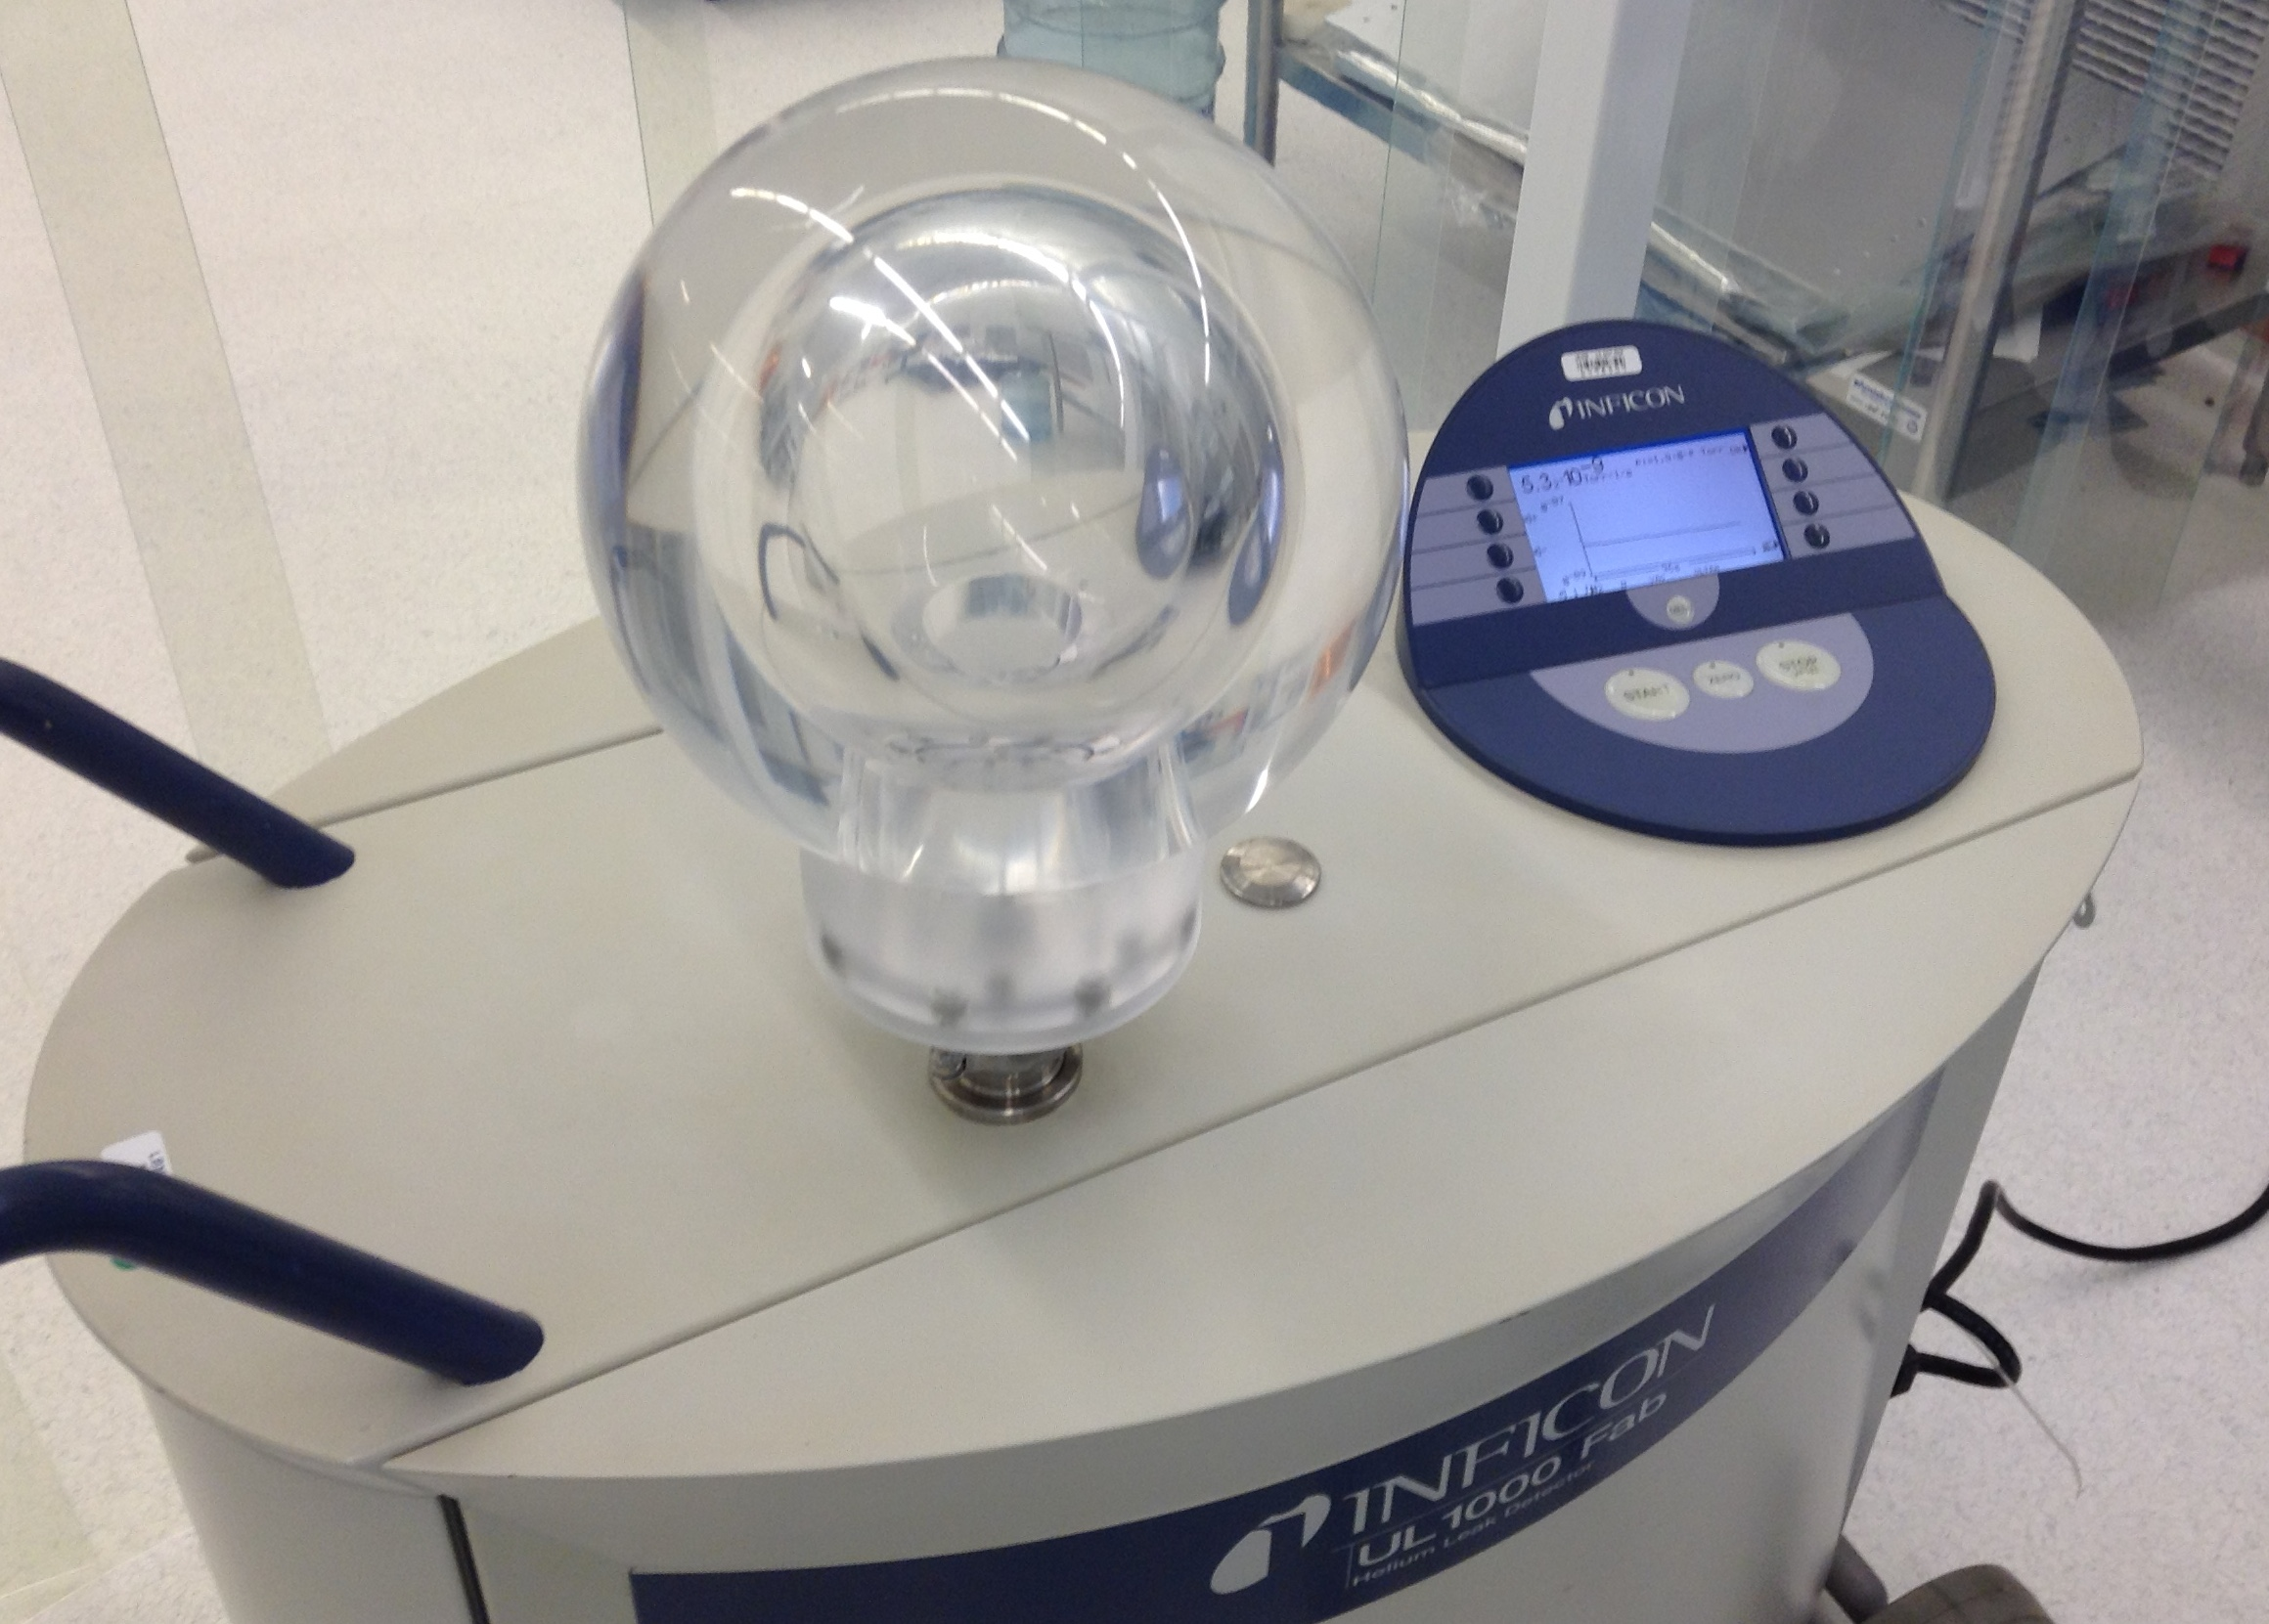
\includegraphics[width=\textwidth]{img_0328.jpg}
                \caption{}
                \label{fig:HeLeakCheckSetup}
        \end{subfigure}%
        \vspace{0.2cm}
        \begin{subfigure}[b]{0.45\textwidth}
                \centering
                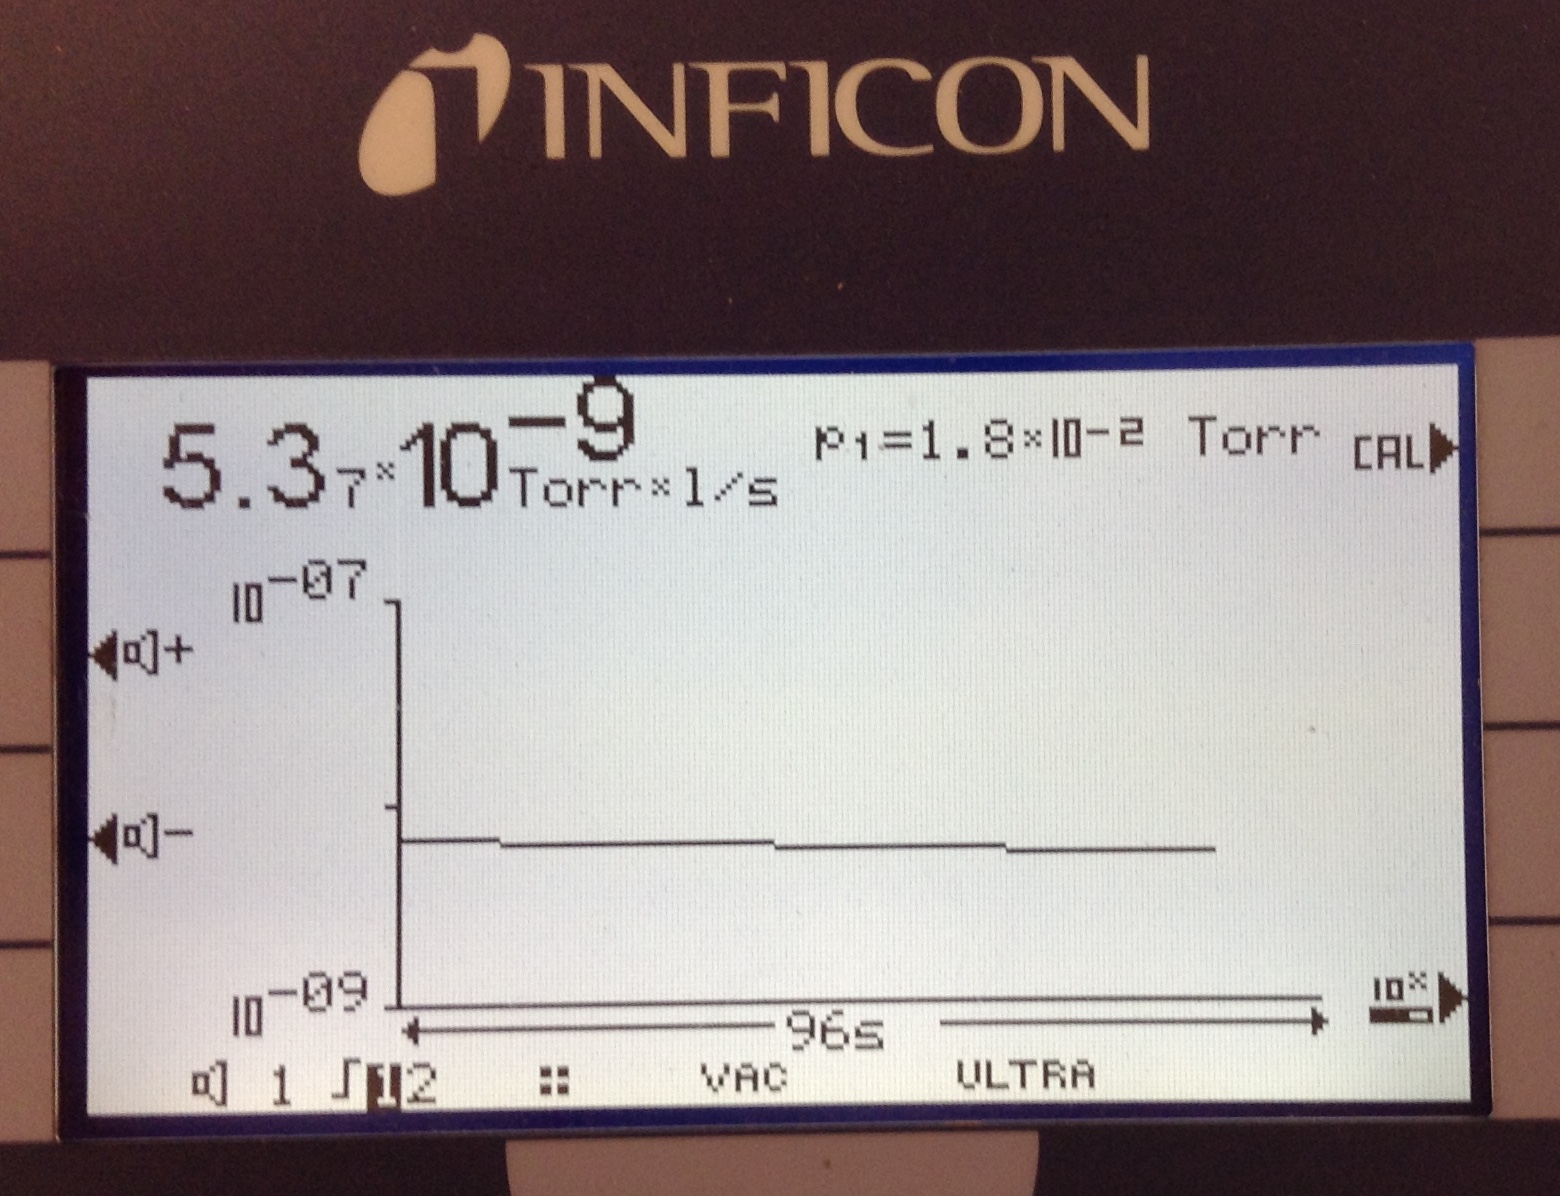
\includegraphics[width=\textwidth]{img_0326.jpg}
                \caption{}
                \label{fig:HeLeakCheckResult}
        \end{subfigure}
        \caption{Helium-leak checking of the decay chamber using INFICON UL1000 in the LBNL clean room.}
\label{fig:HeLeakCheck}
\end{figure}

\subsection{Tag PMT Response}
\label{sec:tagpmt}
The H11432-100 PMT efficiency and gain were measured before and after potting into the PMT assembly both to ensure the PMT had appropriate sensitivity across a wide range of photon fluxes and to see what effect the potting had on the PMT. This was done by placing the PMT in a dark-box 50\,cm away from a calibrated LED. The LED was pulsed for 50\,ns at various voltages to change the photon flux. Figure~\ref{fig:pmttest} shows that the PMT is indeed sensitive over a large range of photon fluxes, however, comparing Figure~\ref{fig:pmttest} to Figure~\ref{fig:pmtafterpotting} shows that the potting of the PMT seems to have reduced the PMT efficiency enough to make tagging single or a few photons less reliable. As we are expecting roughly 20,000 primary scintillation photons this should not be an issue. However, only wavelength-shifted photons will be detectable and the wavelength shifting efficiency quite difficult to evaluate.

\begin{figure}
    \begin{subfigure}{0.49\textwidth}
        \caption{Before potting.}
        \label{fig:pmttest}
        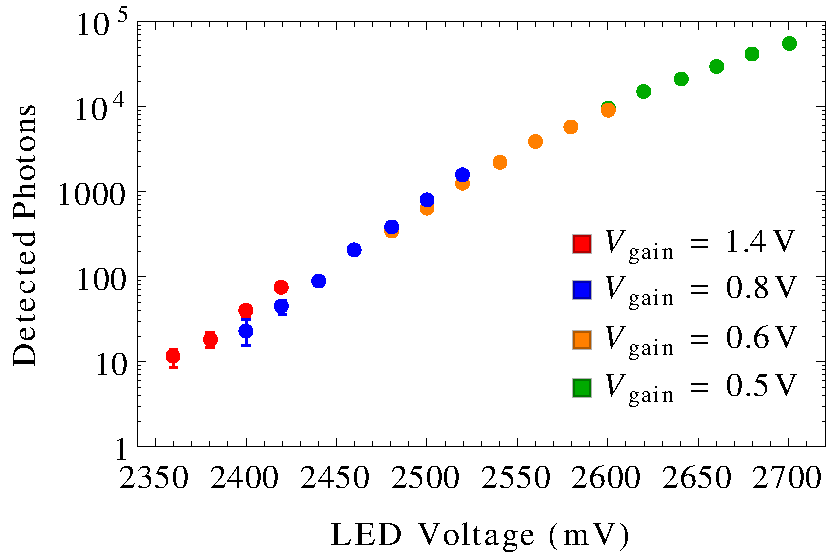
\includegraphics[width=\textwidth]{pmttest}
    \end{subfigure}%
    \begin{subfigure}{0.49\textwidth}
        \caption{After potting.}
        \label{fig:pmtafterpotting}
        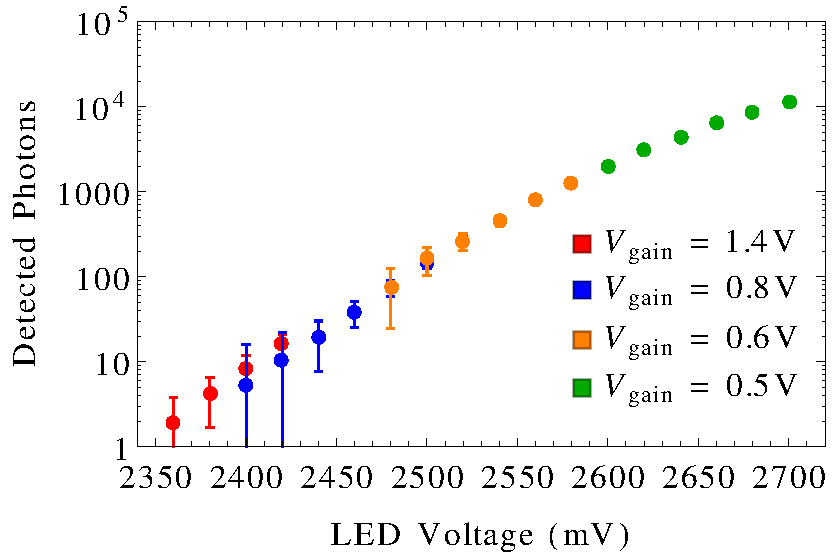
\includegraphics[width=\textwidth]{pmttest_potted}
    \end{subfigure}
    \caption{Tag PMT response measured at various different gains and photon fluxes. A calibrated LED was placed 50\,cm from the face of the PMT and pulsed for 50\,ns at various voltages that produced a known photon flux on the PMT.}
	\label{fig:calibratedled}
\end{figure}

\subsection{Hydrostatic Pressure Test}

The Queen's pressure chamber was used to pressure test all SNO sources and was similarly used to pressure test the Cherenkov source. 
The purpose of this test is to demonstrate the mechanical stability of the source when exposed to pressures consistent with being submerged in SNO+.
This pressure chamber is a 10" diameter aluminum cylinder that is pressurized with tap water pressure. For this test the Cherenkov source was removed from its radon proof bag and fully assembled in a clean room environment with viton o-rings. A 5/8" aluminum plug was used in place of an ubmilical. Because of the use of tap water extra care was taken to ensure the source would not be contaminated by isolating it from the bulk volume of water. The source was heat sealed into a bag of DI water and lowered into the pressure chamber, which was also filled with DI water. After sealing the chamber it was pressurized to 60psi and the source remained at this pressure for one hour. This pressure exceeds the approximately 22psi pressure differential from mine pressure to the bottom of the acrylic vessel by a very conservative margin. To achieve this pressure approximately $0.5\%$ of the water inside the pressure chamber (but outside the sealed bag) was tap water. After depressurizing, the bagged source was removed from the pressure chamber and the bag was inspected to confirm there were no leaks into the tap water contaminated volume. The Cherenkov source was then removed from the DI water bag and was dried externally with grade 5.0 nitrogen gas in a clean room environment. 

To confirm that the Cherenkov source passed the pressure test, the source was disassembled in a clean room environment and inspected for water ingress. Neither the single o-ring seal at the steel-acrylic interface, the double o-ring seal at the umbilical flange, nor the double o-ring seals at the umbilical showed any sign of a water leak. With this result the source passed the pressure test.

\section{Water Phase Analysis}
\label{chap:water_phase}
The Cherenkov source was deployed in SNO+ water phase to calibrate the optical output of the source relative to the \N source.
The following sections describe the deployment effort and the resulting calibration of the source.

\subsection{Data Taking}
In total 18 hours of data were taken with the source deployed and \Li being injected into the decay chamber.
The PMT tag signal was connected to an empty PMT channel of the SNO+ electronics (FECD) to integrate the resulting pulses for event tagging.
In addition, the PMT signal was connected to the trigger signal digitizer (CAEN) in the SNO+ tigger system to record the full pulse.
During this deployment we discovered the gas connections were not ideal for connecting to SNO umbilicals, which leaves some room for improvement for future deployments.

\subsection{Data Cleaning}
In water phase there is no expected scintillation contamination from Bremsstrahlung gammas, however, since the detector is self triggering during deployment, tagged events must be identified and separated from other unrelated detector triggers.
This is done by characterizing the signal from the tag PMT contained within the source.
For a perfect event, the alpha scintillation within the source will result in a large signal with a long time constant.
There is some contamination from \Li betas, which clip the PMT prior to exiting the source, and should be excluded.


\begin{figure}
\centering
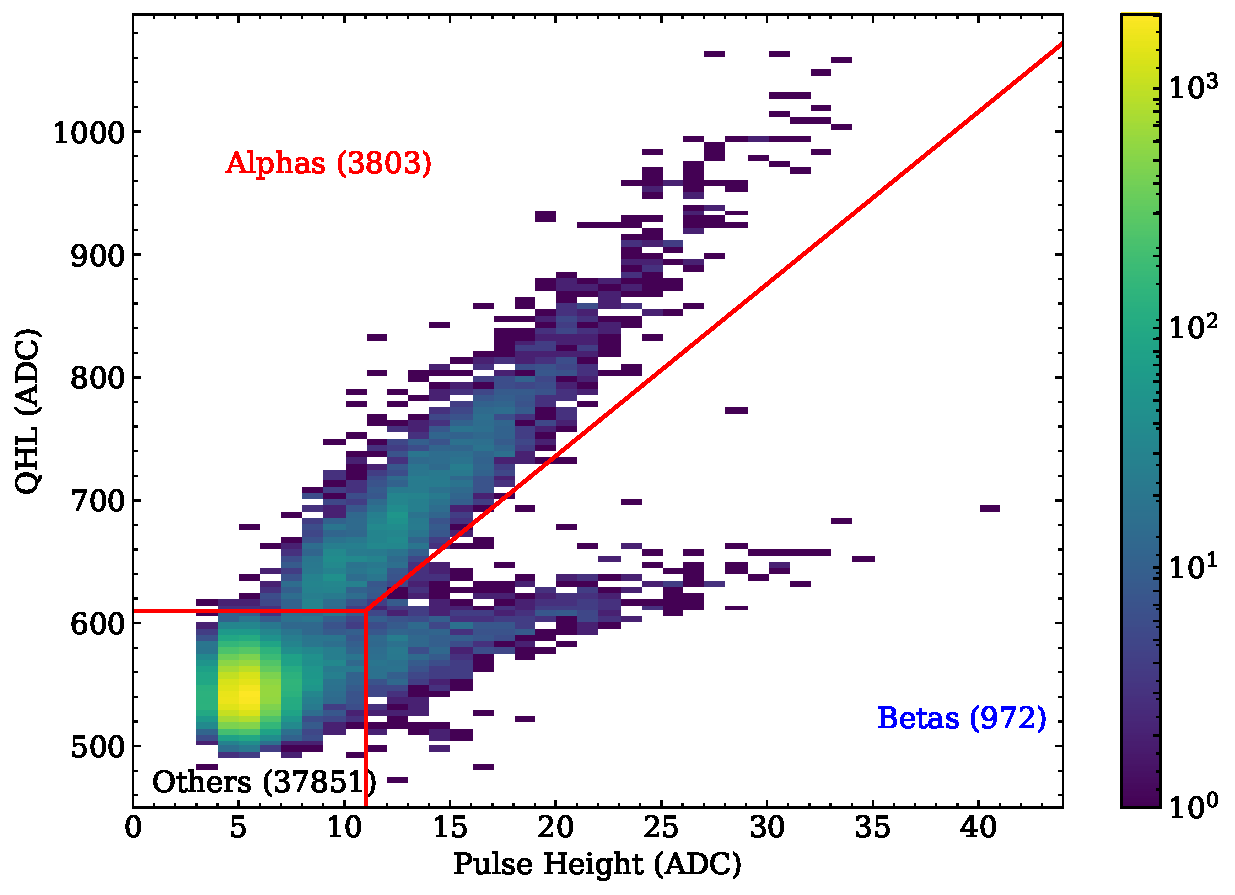
\includegraphics[width=0.8\columnwidth]{data_tagging}
\caption{\label{fig:chsrc_classify} Shown here are all events where the tag PMT crossed threshold during detector triggers during source deployment. Note the tag threshold was set quite low, resulting in a population of ``other" events inconsistent with true alphas or beta contamination. Red lines show nominal cut values used in classification.}
\end{figure}

These events can be well separated in a 2D histogram of total charge (QHL) vs pulse height from the tag PMT. 
Classifications of events with nominal cuts are shown in \Cref{fig:chsrc_classify}.
The population of ``other" events are those in which the detector issued a trigger unrelated to the Cherenkov source, and hence no light was seen by the tag PMT.
The distribution of number of hit PMTs in the detector for each of these classifications is shown in \Cref{fig:chsrc_nhits} while \Cref{fig:chsrc_pmttraces} shows the average digitized trace for each class.
The alphas have an nhit distribution nominally consistent with MC expectations, and a large tag trace with a long tail consistent with alpha scintillation light.


\begin{figure}
\centering
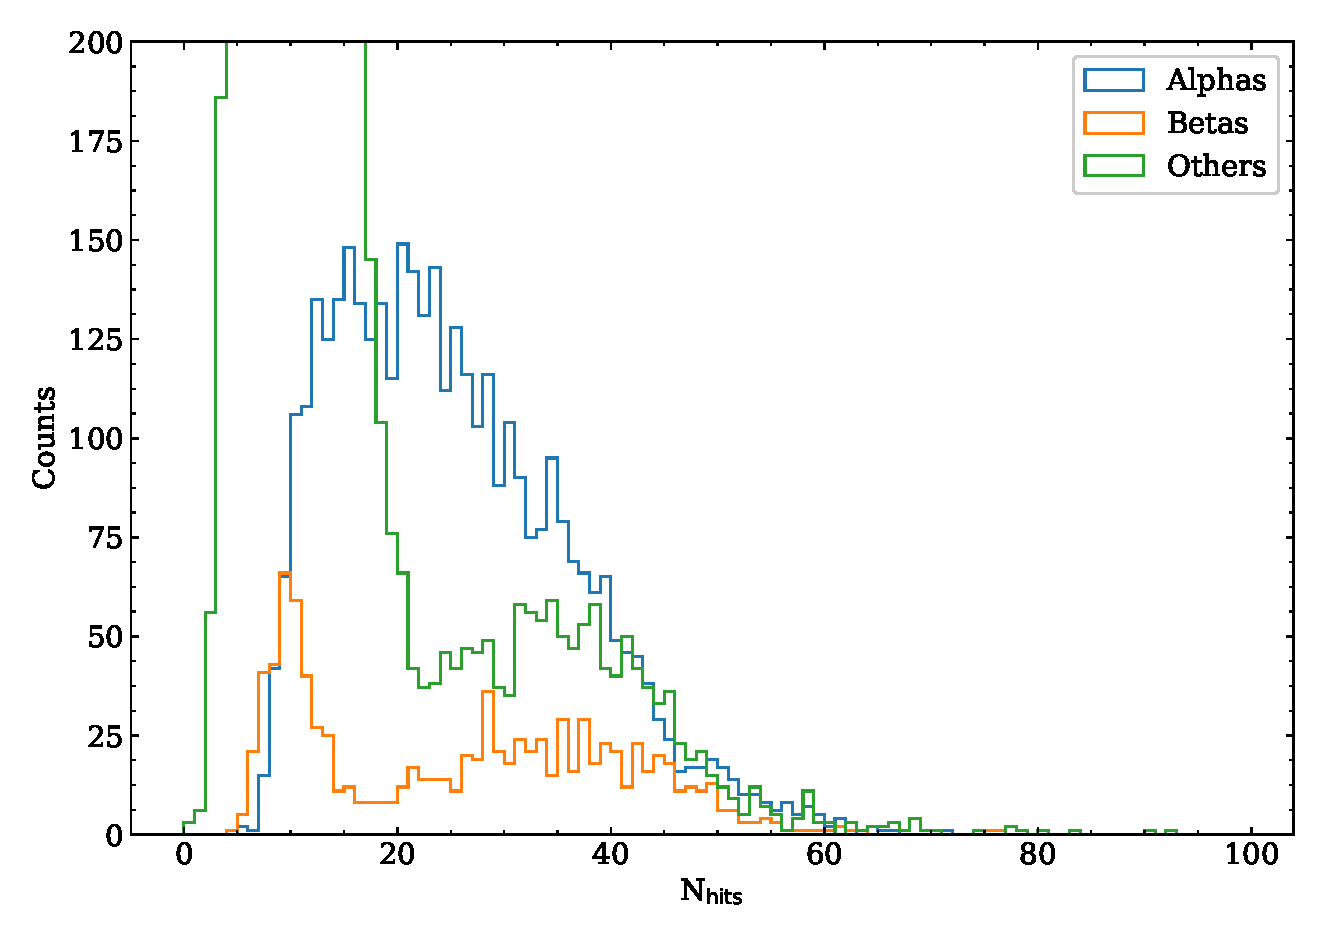
\includegraphics[width=0.75\columnwidth]{nhit_dists}
\caption{\label{fig:chsrc_nhits} The hit PMT distributions for the different classifications of Cherenkov source data.}
\end{figure}


\begin{figure}
\centering
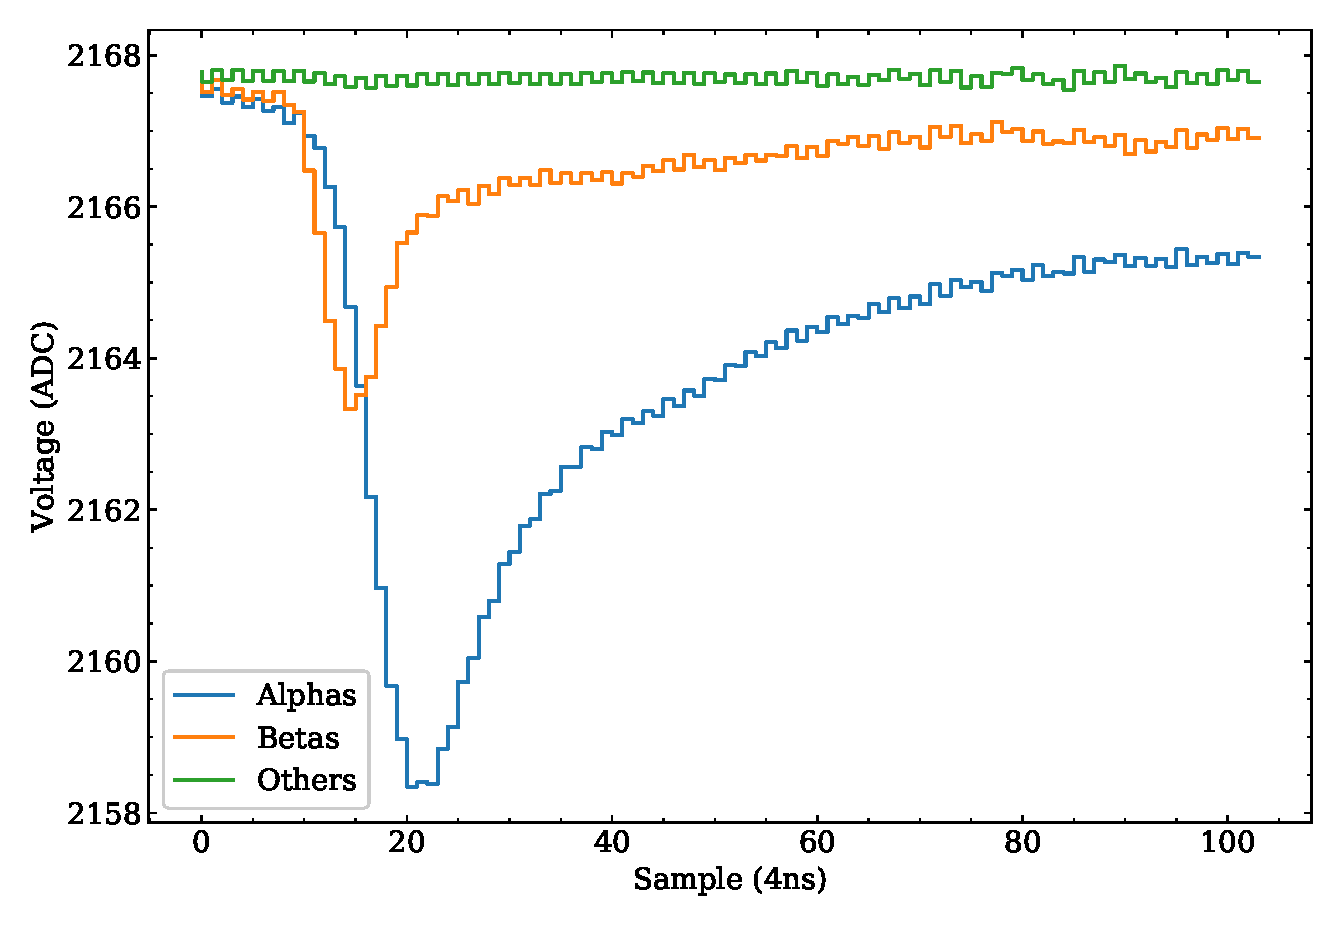
\includegraphics[width=0.75\columnwidth]{average_traces}
\caption{\label{fig:chsrc_pmttraces} The average tag PMT traces from the different classifications of Cherenkov source data.}
\end{figure}

\subsection{Collection Efficiency Fit}
\label{sec:water_fit}
The most straightforward way to extract the correction factor to the MC collection efficiency is to varry that efficiency in MC to maximize the Poisson likelihood of the data.
MC is generated with an \N calibrated photon collection efficiency $C_{eff_0}$.
This quantity is scanned over a range of collection efficiencies while a MC model of the source is used to predict a hit PMT distribution.
To avoid a regime where detector trigger inefficiency is relevant, only events with $>20$ detected photons -- where trigger efficiency is guaranteed to be 100$\%$ -- are included in this analysis.
At each point in the scan the negative logarithm of the Poisson likelihood of the data is calculated resulting in a best fit at $0.945^{+0.015}_{-0.015}$ $C_{eff}/C_{eff_0}$ where the errors are statistical only.
The scan itself is shown in \Cref{fig:chsrc_scan} with the best fit hit PMT distribution in \Cref{fig:chsrc_bestfit}.
This indicates a systematic offset between the light emission of the MC model of the source and the actual source of roughly $5\%$, which should be taken into account when calibrating future phases of SNO+.

\begin{figure}
\centering
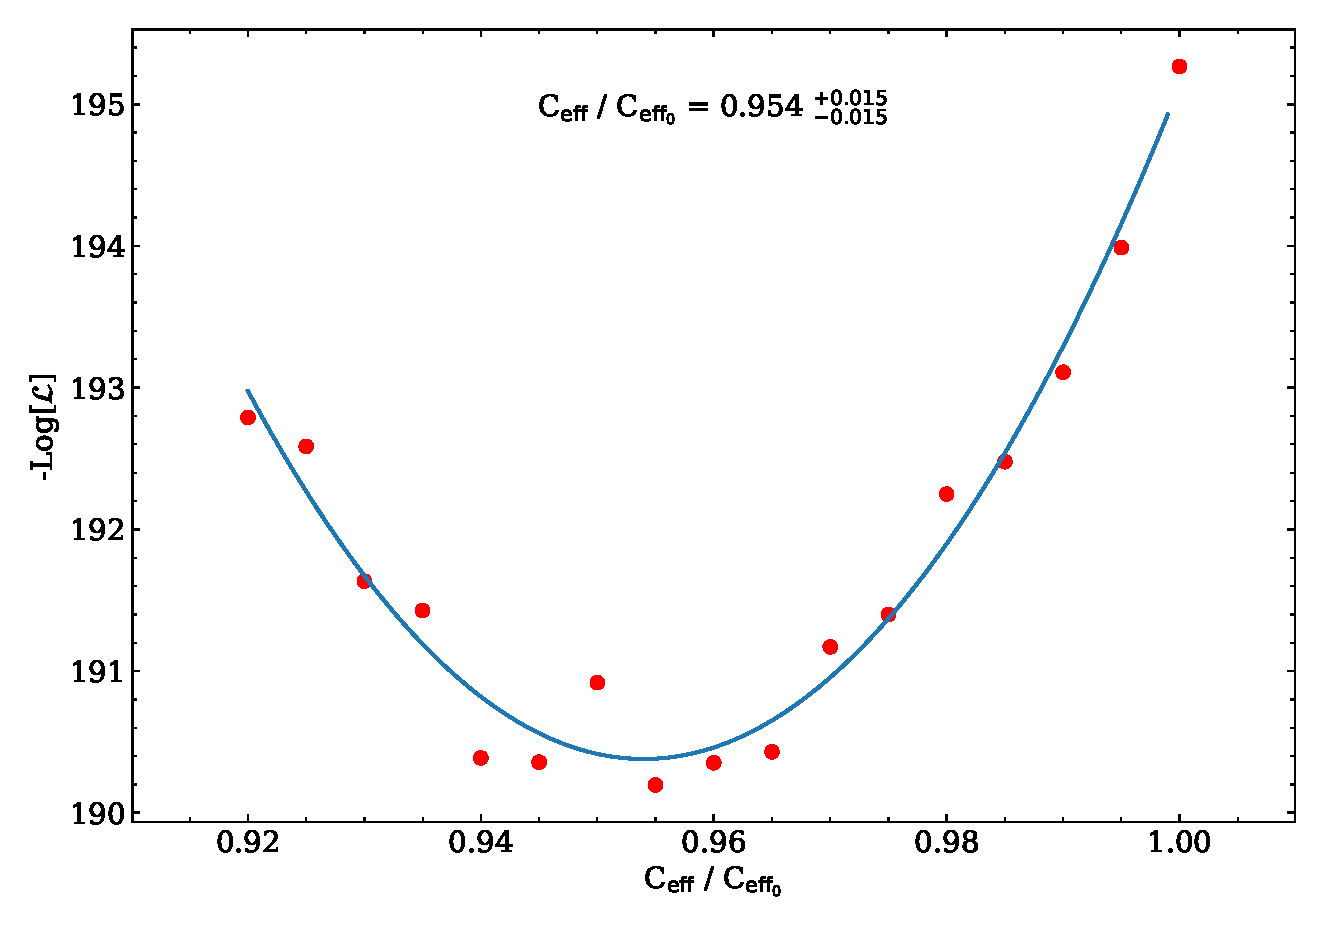
\includegraphics[width=0.75\columnwidth]{100k_bulk_py_ceff_scan}
\caption{\label{fig:chsrc_scan} A plot of the region around the minimmum negative log likelihood space in the collection efficiency scan for calibrating the Cherenkov source.}
\end{figure}

\begin{figure}
\centering
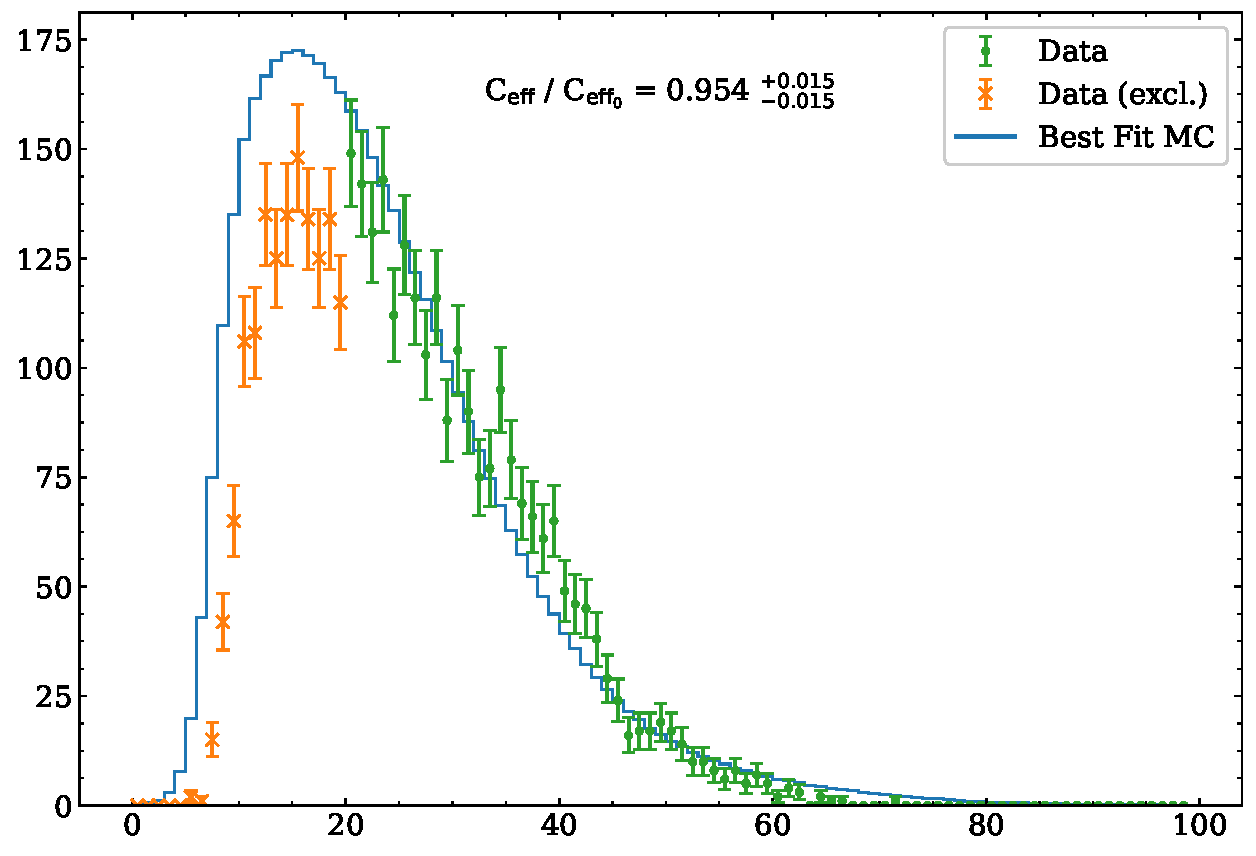
\includegraphics[width=0.75\columnwidth]{100k_bulk_py_ceff_scan_bestfit}
\caption{\label{fig:chsrc_bestfit} A comparison between data and simulation for the best fit collection efficiency in the water phase deployment for the Cherenkov source.}
\end{figure}

Since the MC model is already calibrated relative to the \N source, this systematic offset indicates that the MC model of the Cherenkov source over predicts the production of Cherenkov photons relative to the actual source.
The most likely cause for this is uncertainty in the precise absorption characteristics of the UVA acrylic, which is why this source required calibration.
It is possible that tweaking the source geometry in MC could correct this systematic offset, however, it is sufficient to adjust the MC collection efficiency in future phases to reproduce the measured collection efficiency ratio.


\section{Scintillator Analysis Plan}
The potential of the Cherenkov source in obtaining measures of the overall light collection efficiency in scintillator phase has been investigated using RAT simulations. 
The effect and elimination of scintillation light resulting from unwanted bremsstrahlung gammas was studied.  
In all of the simulations, the Cherenkov source was positioned at the center of the detector, and the source was assumed to be constructed from UV-absorbent (UVA) acrylic.
 
 \begin{figure}
 \begin{subfigure}{.48\textwidth}
   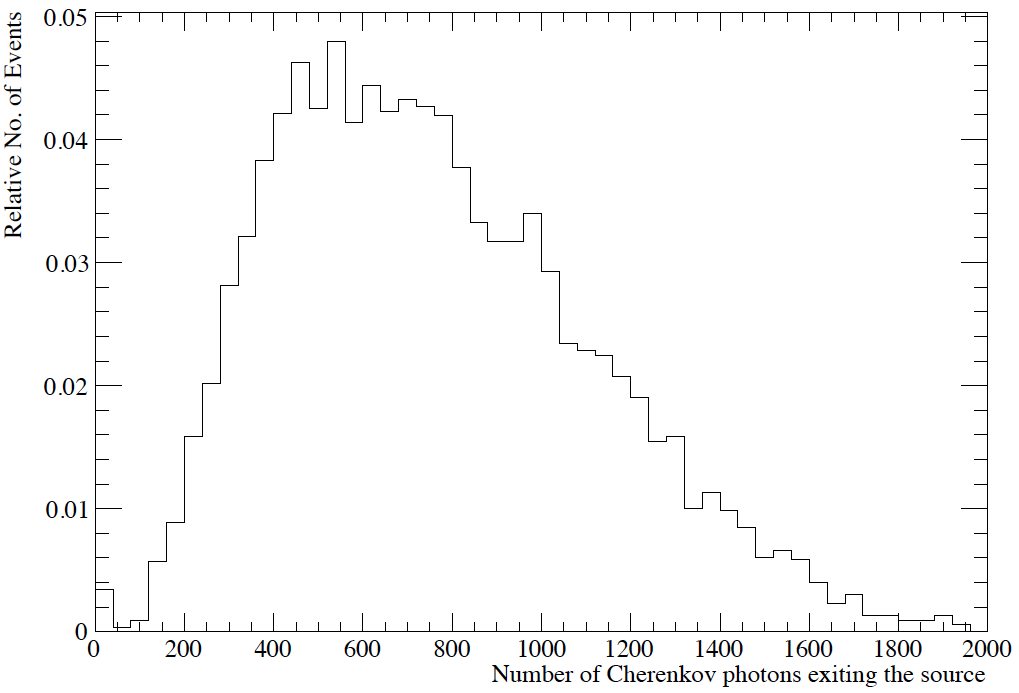
\includegraphics[width=.92\textwidth]{nhit.png}
   \caption{Distribution of number of Cherenkov photons exiting the source for events without scintillation light.}
   \label{fig:nphotons}
 \end{subfigure}
 \hspace{0.5cm}
 \begin{subfigure}{.48\textwidth}
   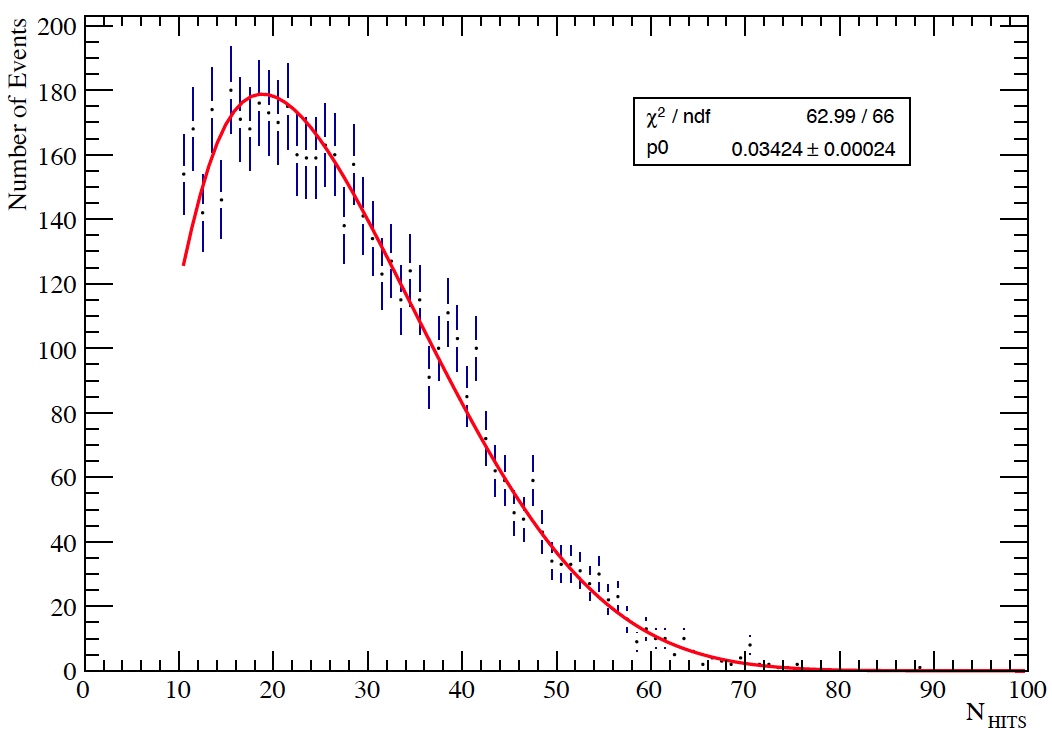
\includegraphics[width=.92\textwidth]{fit.png}
   \caption{Fit of NHit-distribution to sum of binomial distributions.}
   \label{fig:fit}
 \end{subfigure}
 \caption{Using RAT simulations of the Cherenkov source to extract the overall light collection efficiency. Figures taken from~\cite{Heintzelman:2013}. }
 \label{fig:heintzelman-plots}
 \end{figure}
 
\subsubsection{Cutting Bremsstrahlung Events}

The decay of \Li in the Cherenkov source produces betas with an end-point energy of about 13\,MeV. 
In addition to producing Cherenkov light in the acrylic, bremsstrahlung gammas are also produced in a significant number of events.  
These gammas exit the source and are likely to Compton-scatter in the scintillator inside the AV.  
Simulations indicate that Compton-scatter electrons are produced in about 1/3 of the events.  
With scintillator as the target, these events produce much more light and, importantly, have timing profile consistent with scintillation events instead of water.  
Because the light output from such events is more indicative of scintillator properties than detector response, it is desirable to eliminate such bremsstrahlung events from the dataset.
For this, a cut based on the likelihood ratio of the distribution of PMT hit-time residuals was found to be particularly effective, due to the very different time profiles of scintillation and Cherenkov light.

\subsubsection{Extracting the light Collection Efficiency}
The distribution of the number of photons exiting the Cherenkov source per non-scintillation event are predicted by simulation, see Figure~\ref{fig:nphotons}. 
Using this information, the total probability of observing a certain number of hits is fitted to the distribution of the detected number of photons for simulated events as shown in Figure~\ref{fig:fit}.
This method can extract the total photon detection probability, however, as was discovered in the water phase analysis, the true quantity of interest is the correction to the MC collection efficiency necessary to result in a calibrated simulation.
The analysis described for water phase in \Cref{sec:water_fit}, with the additional removal of bremsstrahlung events, can be repeated here to calibrate RAT once scintillator data exists for the Cherenkov source.
